%% Based on techreport.tex template as sent by Erik Burger on 2023-11-20
%% 
%% Karlsruhe Institute of Technology
%% Institute for Program Structures and Data Organization
%% Chair for Software Design and Quality (SDQ)
%%
%% Dr.-Ing. Erik Burger
%% burger@kit.edu
%%
%% See https://sdq.kastel.kit.edu/wiki/Dokumentvorlagen
%%
%% Version 1.0, 2023-11-20

%% Available page modes: oneside, twoside
%% Available languages: english, ngerman
%% Available modes: draft, final (see README)
\documentclass[oneside, ngerman]{sdqtechreport}

%% ---------------------------------
%% | Information about the document |
%% ---------------------------------

%% Name of the group and authors
\author{Paul Buda, Martin Scheuermann, Stephan Schneider, \\
Simon Schütz und Nils Seibert}

%% Title (and possibly subtitle) of the thesis
\title{Pflichtenheft}

\subtitle{zur Android-App Neptune}

%% You can put a logo in the ``logos'' directory and include it here
%% instead of the SDQ logo
% \grouplogo{myfile}
%% Alternatively, you can disable the group logo
% \nogrouplogo

\date{01.12.2023}

%% For example texts -- please remove in the final version
\usepackage{blindtext}

%% ====================================
%% ====================================
%% ||                                ||
%% || Beginning of the main document ||
%% ||                                ||
%% ====================================
%% ====================================
\begin{document}

%% Set PDF metadata
\setpdf

%% Set the title
\maketitle

%% ------------------------
%% |   Table of Contents  |
%% ------------------------
\tableofcontents

%% -----------------
%% |   Main part   |
%% -----------------
\cleardoublepage

%% -------------------
%% | Example content |
%% -------------------

\chapter{Einleitung}
\label{chap:Einleitung}

\section{Einführung}
\label{sec:Einleitung:Einführung}
Musik spielt im Leben vieler Menschen eine enorm wichtige Rolle. Insbesondere bei Partys und Zusammenkünften mit Freunden sorgt eine gute Musikauswahl für eine gute Stimmung unter den Anwesenden. Aber auch der umgekehrte Fall ist vielen sicherlich gut bekannt – gefällt die abgespielte Musik den Anwesenden nicht, so kann dies die Stimmung erheblich trüben.

Nahezu alle der heute gängigen Musikstreaming-Anbieter versuchen bereits mit proprietären Lösungen, dem entgegenzuwirken. In der Praxis jedoch sind die eigens von den Anbietern angebotenen Lösungen häufig nicht praktikabel. Die Ursachen hierfür sind divers, so setzen die von den Anbietern selbst entwickelten Tools häufig voraus, dass alle Teilnehmer über ein bestehendes Abonnement beim entsprechenden Anbieter verfügen. 

Das Ziel des Projekts ''Neptune'' ist es, eine praktikable Lösung für die eingangs beschriebene Problematik anzugeben. Hierzu soll im Rahmen des Moduls ''Praxis der Softwareentwicklung'' eine Android-App entwickelt werden, mithilfe derer über die bei einer Party oder einem vergleichbaren Event abgespielte Musik entschieden werden kann.

Hierzu sollen die Anwesenden in verschiedenen verfügbaren Abstimmungs-Modi Musikvorschläge einbringen und über diese abstimmen können. Die Musik soll dann über das Endgerät einer weiteren anwesenden Person, des sogenannten ''Hosts'', abgespielt werden. 
Mittels der Einbindung eines gängigen Musikstreaming-Service soll die App in die Lage versetzt werden, einen breiten Musikkatalog bereitzustellen.


\section{Anwendungsbereich}
\label{sec:Einleitung:Anwendungsbereich}

Das Ziel von Neptune ist es, die Musikauswahl bei privaten Veranstaltungen, wie zum Beispiel studentische WG- und Wohnheimpartys, einfacher und gerechter zu gestalten.
Die Android-App Neptune bietet Gruppen die Möglichkeit jeden an der Musikauswahl zu beteiligen und über die Abspielreihenfolge demokratisch abzustimmen. Durch die Integration mit einem Audio-Streaming-Dienst wie Spotify kann Neptune automatisch die am besten bewerteten Tracks abspielen. Damit ist es möglich Songwünsche von Gästen zu erfüllen, ohne einen aktiven ''DJ''  der die Wünsche entgegen nimmt und sie manuell in die Warteschlange hinzufügt.

Bei der Erstellung einer Session kann der Gastgeber die verfügbaren Tracks nach Belieben auf verschiedene Genres/Artists oder eine Playlist beschränken. Nach Auswahl des Modus kann der Gastgeber die Gäste einladen, sich an der Musikauswahl zu beteiligen, indem er einen sechsstelligen Zahlencode oder einen Link weitergibt. Die Gäste können dann in der App Tracks in die Vorschlagsliste hinzufügen und mit dem Verteilen von Upvotes Lieder in der Liste nach oben voten und sie somit schneller zum Abspielen bringen. Der Host hat durch eine Kontrollansicht einen Überblick über die Queue, sowie die Vorschlagsliste in Neptune. Er kann in dieser Ansicht Tracks in die Queue hinzufügen und entfernen, sowie Tracks aus der Vorschlagsliste sperren, dadurch hat der Host weiterhin die volle Kontrolle über die Musikauswahl. Zusätzlich kann er durch die Einstellung
eines Cooldowns verhindern, dass diesselben Tracks mehrmals mit geringen Abstand gespielt werden.

Eine vollständige Beschreibung der Anwendungsfälle sind  den \hyperlink{Anwendungsfaelle}{Use Case Diagrammen} zu entnehmen   


\section{Zielgruppe}
\label{sec:Einleitung:Zielgruppe}

Die primäre Zielgruppe von Neptune besteht aus Veranstaltern und Besuchern von Privatpartys, die zwischen 5-50 Besucher haben. Das Alter der Zielgruppe liegt dabei bei 18-35 Jahren, in dieser Altersgruppe ist von Vertrautheit bei der Bedingung von Smartphoneapps auszugehen. Darüber hinaus haben eine Mehrheit in dieser Altersgruppe einen Zugang zu Spotify, sowie ein aktuelles Smartphone. Dadurch sind die Zugangsbarrieren für die Benutzung von Neptune sehr niedrig.

Auch für Menschen außerhalb dieser primären Zielgruppe kann Neptune durch sein flexibles und einfaches Design interessant sein. Zum Beispiel ist es mit der App auch möglich, über die perfekte Entspannungsmusik beim Yoga abzustimmen oder das beliebteste Weihnachtslied in der Großfamilie zu ermitteln. 
Im Rahmen dieses PSE-Projekts wird die Zielgruppe auf Androidbenutzer eingeschränkt.

\chapter{Zielbestimmungen}
\label{chap:Zielbestimmungen}

\section{Musskriterien}
\label{sec:Zielbestimmungen:Musskriterien}
\begin{itemize}
    \item Mithilfe des Systems sollen User gemeinsam auf Veranstaltungen live über die während der Veranstaltung abgespielte Musik abstimmen bzw. entscheiden können.
    \item Hauptbestandteil des Systems ist ein Abstimmungssystem, welches Participants das Vorschlagen von Tracks ermöglicht. Dazu stellt das System verschiedene Modi zu Auswahl.
    \begin{itemize}
        \item Participants können Tracks maximal ein Upvote abgeben. Je nach gewähltem Abstimmungsmodus hat die jeweilige Anzahl der Upvotes eines Tracks Einfluss darauf, ob und wann er abgespielt wird.
    \end{itemize}
    \item Das System ist in der Lage, Usern einen durchsuchbaren Musikkatalog zur Verfügung zu stellen. Diese werden über entsprechende, auf dem Markt verfügbare Schnittstellen externer Anbieter bereitgestellt. Konkret wird dies im System durch die Einbindung mindestens einer externen API-Schnittstelle eines Musikstreaming-Anbieters realisiert.
    \begin{itemize}
        \item Das im Rahmen des Moduls ''Praxis der Softwareentwicklung'' zu entwickelnde System beschränkt sich hierbei auf einen konkreten Musikstreaming-Anbieter, namentlich auf das Angebot des schwedischen Unternehmens Spotify. Hierbei soll die Möglichkeit zur einfachen komplexen Ausweitung des Systems auf weitere Musikstreaming-Anbieter gegeben sein.
        \begin{itemize}
            \item Aufgrund von Einschränkungen seitens Spotify bezüglich der Entwicklerarbeit mit der von Spotify bereitgestellten API ist die vorgesehene Anzahl zulässiger User innerhalb einer gemeinsamen Session zunächst auf 25 User beschränkt.
            \item Aufgrund der Eigenschaften der Spotify-API ergibt sich darüber hinaus, dass für User ohne Spotify-Account sowie User ohne einen Spotify-Account mit einem Premium-Abonnement vorgesehen ist, dass diese nicht selbst neue Tracks in der App vorschlagen können. Jedoch können diese User über von anderen Usern vorgeschlagene Songs abstimmen.
        \end{itemize}

    \end{itemize}
    \item Für eine Veranstaltung kann eine sogenannte Session durch den Host erstellt werden. Participants können dieser mithilfe eines sechsstelligen Beitrittscodes beitreten. Alle Entscheidungen über abzuspielende Musik finden innerhalb der Session statt.
    \item Das System verwendet zur Entscheidung über abzuspielende Songs ein nach diversen Kriterien konfigurierbares Abstimmungssystem.
    \begin{itemize}
        \item Zum einen sind verschiedene Abstimmungsmodi vorgesehen:
        \begin{itemize}
            \item General Mode
            \begin{itemize}
                \item Full Participants sowie der Host können im bereitgestellten Musikkatalog einen beliebigen Track auswählen und diesen durch einen Upvote vorschlagen
                \item Participants haben die Möglichkeit, einem Track ein Upvote zu geben. Hat ein Participant bereits selbst ein Upvote an einen Track vergeben, so ist es ihm möglich, diesen wieder zu entfernen.
                \item Der Host kann einen Track, welcher ein Upvote erhalten hat, zur Queue hinzufügen. Außerdem hat er die Möglichkeit, Tracks zu sperren.
            \end{itemize}
            \item Artist Mode
            \begin{itemize}
                \item Die Grundfunktionalität ist gleich der des General Modes. Hierbei legt der Host jedoch zuvor eine Liste an erlaubten Artists fest. Während der gesamten Session kann ein Track ausschließlich dann in der Suche gefunden, vorgeschlagen werden, Upvotes erhalten und abgespielt werden, wenn er mindestens einem der erlaubten Artists zugeordnet werden kann.
            \end{itemize}
            \item Genre Mode
            \begin{itemize}
                \item Die Grundfunktionalität ist gleich der des General Modes. Hierbei legt der Host jedoch zuvor eine Liste an erlaubten Genres fest. Während der gesamten Session kann ein Track ausschließlich dann in der Suche gefunden, vorgeschlagen werden, Upvotes erhalten und abgespielt werden, wenn er mindestens einem der erlaubten Genres zugeordnet werden kann.
            \end{itemize}
            \item Playlist Mode
            \begin{itemize}
                \item Die Grundfunktionalität ist gleich der des General Modes. Hierbei hinterlegt der Host jedoch zuvor eine Playlist, welche von dem für die Session genutzten Musikstreaming-Anbieter stammt. Während der gesamten Session kann ein Track ausschließlich dann in der Suche gefunden, vorgeschlagen werden, Upvotes erhalten und abgespielt werden, wenn er in der hinterlegten Playlist enthalten ist.
            \end{itemize}
        \end{itemize}

    \end{itemize}
    \item Die User können genau eine der untenstehend aufgeführten Rollen bekleiden. Je nach der individuellen Ausgestaltung der Abstimmungsmodi ist die Rolle eines Users entscheidend in Hinblick auf die Entscheidungsfindung zur abzuspielenden Musik.
    \begin{itemize}
        \item Host: Der Host ist der Ersteller einer Session. Auf der einen Seite verwaltet er sie und kann sie auflösen, auf der anderen Seite wird die abzuspielende Musik über sein Endgerät abgespielt.
        \item Participant: Alle Teilnehmer einer Session, welche nicht der Host sind, bekleiden automatisch die Rolle Participant. Participants können basierend auf den gewählten Abstimmungsparametern neue Songs vorschlagen und/oder über vorgeschlagene Songs abstimmen. 
    \end{itemize}
    \item Die abzuspielende Musik wird über externe Anbieter abgespielt. Hierbei wird analog zur Einbindung von Musikstreaming-Anbietern bereitgestellter externer Schnittstellen vorgegangen.
    \item  Für das User Interface der App werden die Sprachen Deutsch und Englisch verwendet. Die Sprachauswahl erfolgt hier automatisch anhand der vom Gerät festgelegten Systemsprache. Ist diese Deutsch, so wird in der App auch Deutsch verwendet. Wird auf dem Endgerät eine andere Sprache als Deutsch als Systemsprache verwendet, so wird in der App automatisch Englisch verwendet.
\end{itemize}

\hypertarget{Wunschkriterien}{}
\section{Wunschkriterien}
\label{sec:Zielbestimmungen:Wunschkriterien}

\begin{itemize}
    \item Jeder User soll in einer Statistikansicht Informationen über die Session einsehen können. Diese Ansicht wird automatisch beim Verlassen der Session angezeigt. Während der Session kann sie durch ein Button geöffnet werden. Die Statistik soll als Bild exportierbar und teilbar sein. 
    Folgende Datenpunkte sollen dabei angezeigt werden. 
    \begin{itemize}
        \item Song mit meisten Votes der Session
        \item Genre mit den meisten Votes der Session
        \item Artist mit den meisten Votes der Session
        \item Anzahl abgespielte Songs in der Session
        \item Dauer der Session
        \item Anzahl Teilnehmer in der Session 
        \item Verteilte Herzen in Session
    \end{itemize}
  
    \item Im Falle dessen, dass die Teilnehmer keine neue Musik vorschlagen und die Warteschlange hierdurch leer ist, soll die App mittels einer Autoplay-Funktion dennoch kontinuierlich Musik abspielen.
    \item QR-Code zum Einscannen, als Erweiterung zum 6 stelligen Beitrittscode

\end{itemize}

\section{Abgrenzungskriterien}
\label{sec:Zielbestimmungen:Abgrenzungskriterien}
\begin{itemize}
    \item Musik soll nicht innerhalb der App selbst abgespielt werden.
    \item Im Rahmen des Projekts soll keine öffentlich zugängliche API und insgesamt keine Schnittstelle für weitere externe Anwendungen bereitgestellt werden
    \item Die App soll, abgesehen von einer Internetverbindung, keine weiteren alternativen Netzwerktechnologien wie Bluetooth o.ä. nutzen.
    \item Die App unterstützt nur den Portrait-Modus, nicht den Landscape-Modus.

\end{itemize}




\chapter{Benutzeroberfläche und funktionale Anforderungen}
\label{chap:Benutzeroberfläche}

\section{Allgemeines}
\label{sec:Benutzeroberfläche:Allgemeines}
Die Benutzeroberfläche wird so gestaltet, dass diese einfach, intuitiv und ohne Vorkenntnisse von Nutzern der Zielgruppe verwendet werden kann. Näheres findet sich unter Benutzerfreundlichkeit im Kapitel Qualitätszielbestimmungen (\ref{Qualitätszielbestimmungen_Benutzerfreundlichkeit}).


\section{Grafikentwürfe und deren funktionale Anforderungen}
\label{sec:Benutzeroberfläche:Grafiken}
% do not show subsections in contents
\addtocontents{toc}{\protect\setcounter{tocdepth}{1}}

Die folgenden Grafikentwürfe sind nur erste Entwürfe. Sie sollen einen ersten Eindruck vom Aussehen der App vermitteln und vor allem die ''Topologie'' der App darstellen: Das heißt, welche Buttons existieren und was diese bewirken. Wir möchten ausdrücklich klarstellen, dass wir die hier gezeigten Designs hinsichtlich Formen, Farben, Anordnung und exakter Beschriftung noch verändern wollen und werden. Die Designs sind nicht als final zu verstehen.

In den folgenden Unterkapiteln finden sich alle Views der App. Der Unterkapitelaufbau ist folgendermaßen: Jede View enthält einen Grafikentwurf und die detaillierte Definition aller wichtigen Benutzeroberflächen-Elemente. Das Klicken selbst und das Verhalten der gesamten Benutzerberfläche nach dem Klicken auf ein klickbares solches Element (<Button> oder <Eingabefeld>) ist stets als funktionale Anforderung zu verstehen. Jedes Klicken ist als Testfall zu verstehen und mit einer entsprechend F-Nummer versehen.
\vspace{\baselineskip} \\

Aufgrund der häufigen Verwendung einer <Track-Liste> wird dieses komplexe Benutzeroberflächenelement an dieser Stelle grundsätzlich definiert:
\vspace{\baselineskip} \\
\textbf{<Track-Liste>:}
\begin{itemize}
    \item Eine Track-Liste ist eine Anzeige für eine Sammlung beliebig vieler Tracks. Die anzuzeigende Sammlung ist jeweils im Einzelnen näher definiert.
    \item Jeder Track wird mit Cover, Titel, Interpret und der Anzahl der Upvotes angezeigt.
    \item Tracks die sich auf der Liste von durch den Host gesperrten Tracks befinden oder einen aktiven Cooldown haben, werden ausgegraut angezeigt. Ihr Upvote-Button ist nicht funktionsfähig.
    \item Eine Track-Liste ist grundsätzlich nicht klickbar, die Anzeige jedes Tracks enthält aber klickbare Buttons:
    \begin{itemize}
        \item <Button> Upvote (immer vorhanden): Beim Klicken des Upvote-Buttons fügt der User dem Track einen Upvote hinzu, falls er den Track noch nicht geupvotet hat. Ansonsten wird durch das Klicken der Upvote entfernt. Dabei ändert sich das Aussehen des Upvote-Buttons, um den derzeiten Upvote-Zustand anzuzeigen.
        \item <Button> Track-Menü (nur in Track-Listen für den Host vorhanden): Beim Klicken des Track-Menu-Buttons öffnet sich ein Dropdown-Menü mit Auswahlmöglichkeiten, die entsprechende Funktionalitäten besitzen. Diese Auswahlmöglichkeiten sind jeweils im Einzelnen näher definiert.
    \end{itemize}
    \item Bei Track-Listen für den Host kann eine Drag-and-Drop-Funktionalität implementiert sein. Diese ist jeweils im Einzelnen näher definiert.
    \item Die Track-Liste ist scrollbar.
\end{itemize}


\subsection{Startseite (startView)}
\label{sec:Benutzeroberfläche:startView}

\begin{center}
    \hypertarget{startView}{}
    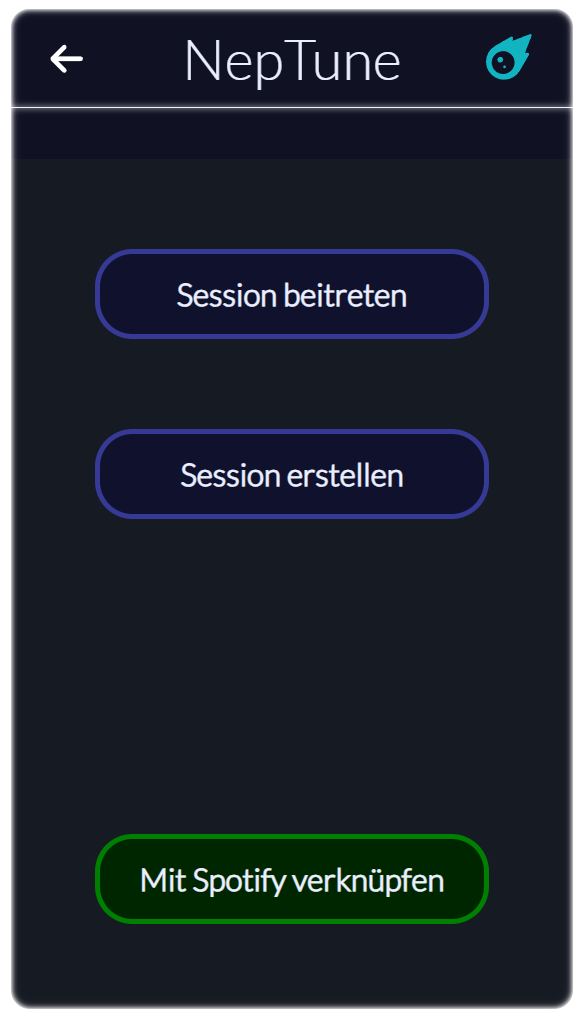
\includegraphics[width=0.4\textwidth]{LATEX/Pflichtenheft/GraphicDesigns/startPage.png}
    \captionof{figure}{startView}
\end{center}

\textbf{<Button> Session beitreten:}
\begin{itemize}
    \item Solange der User sich nicht mit einem Spotify-Account verknüpft hat, wird unter dem Button ein Hinweis angezeigt, dass User ohne verknüpften Account nur über die von anderen Usern vorgeschlagene Tracks abstimmen können. Zum Vorschlagen neuer Tacks wird ein verknüpfter Spotify-Account benötigt.
    \item <F 1.1> Durch Klicken des Buttons ''Session beitreten'' gelangt der User auf die \hyperlink{joinSessionView}{joinSessionView}. Dabei wird er zum Full Participant, wenn er mit einem Spotify-Account verknüpft ist. Anderfalls wird er zu einem Restricted Partcipant.
\end{itemize}

\textbf{<Button> Session erstellen:}
\begin{itemize}
    \item Der Button ''Session erstellen'' ist so lange deaktiviert und verblasst, bis sich der User über den Button ''Mit Spotify verknüpfen'' erfolgreich mit einem Spotify-Premium-Account verknüpft hat. Danach wird der Button funktionsfähig.
    \item Solange der Button ''Session erstellen'' deaktiviert ist, wird darunter ein Hinweis angezeigt, dass das Erstellen einer Session nur mit einem verknüpften Spotify-Premium-Account möglich ist.
    \item <F 1.2> Durch Klicken des funktionsfähigen Buttons ''Session erstellen'' gelangt der User auf die \hyperlink{hostModeSelectView}{hostModeSelectView}.
\end{itemize}

\textbf{<Button> Mit Spotify verknüpfen / Von Spotify trennen:}
\begin{itemize}
    \item <F 1.3.A> Durch Klicken des Buttons ''Mit Spotify verknüpfen'' verknüpft sich die App, wenn möglich automatisch und im Hintergrund mit dem lokal angemeldeten Spotify-Account. Ist dies nicht möglich öffnet sich die von Spotify zur Verfügung gestellte Anmeldemaske, um per Login seinen Account zu verknüpfen.
    \item Nach dem erfolgreichen Verknüpfen mit Spotify, ändert sich die Beschriftung des Buttons von ''Mit Spotify verknüpfen'' zu ''Von Spotify trennen''.
    \item <F 1.3.B> Durch Klicken des Buttons ''Von Spotify trennen'' wird das Spotify Konto des Users wieder von NepTune getrennt.
    \item Nach dem erfolgreichen Trennen von Spotify, ändert sich die Beschriftung des Buttons von ''Von Spotify trennen'' zu ''Mit Spotify verknüpfen''.
\end{itemize}

\textbf{<Button> Zurück:}
\begin{itemize}
    \item <F 1.4> Beim Klicken des Zurück-Buttons erscheint ein Pop-Up Fenster mit der Frage ''NepTune wirklich schließen?''. In diesem Pop-Up kann sich der User nun zwischen ''Ja'' und ''Nein'' entscheiden.
    \begin{itemize}
        \item <F 1.4.A> Durch Auswählen von ''Ja'' verlässt der User die App und die App wird beendet.
        \item <F 1.4.B> Durch Auswählen von ''Nein'' bleibt der User in der \hyperlink{startView}{startView}.
    \end{itemize}
\end{itemize}



\subsection{Sessionbeitritt (joinSessionView)}
\label{sec:Benutzeroberfläche:joinSessionView}


\begin{center}
    \hypertarget{joinSessionView}{}
    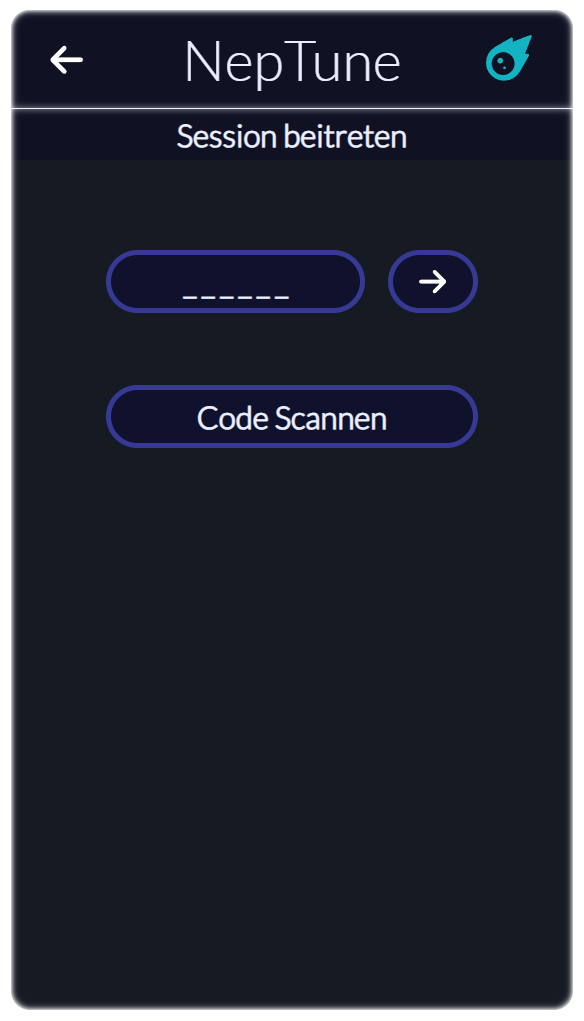
\includegraphics[width=0.4\textwidth]{LATEX/Pflichtenheft/GraphicDesigns/userJoinGroupPage.png}
    \captionof{figure}{joinSessionView}
\end{center}

\textbf{<Eingabefeld> Code-Eingabe:}
\begin{itemize}
    \item Eingabefeld zur Eingabe des sechsstelligen Codes, der die Session eindeutig identifiziert.
    \item <F 2.1> Durch Anklicken des Code-Eingabefelds öffnet sich bei dem User die ''Ziffernblock-Tastatur'', mit welcher der User nun den sechsstelligen Code eingeben kann.
\end{itemize}

\textbf{<Button> Code bestätigen:}
\begin{itemize}
    \item <F 2.2.A> Existiert eine Session zum eingegebenen sechsstelligen Code, führt Klicken des Bestätigungsbuttons auf die \hyperlink{sessionVoteView}{sessionVoteView} der Session.
    \item <F 2.2.B> Existiert keine Session zur Eingabe, erscheint ein entsprechender Hinweis unter dem Code-Eingabefeld und der Inhalt des Code-Eingabefeldes wird gelöscht.
\end{itemize}

\textbf{<Button> Code scannen:}
\begin{itemize}
    \item <F 2.3> Durch Klicken des Buttons ''Code scannen'' öffnet sich ein QR-Code-Reader. Nach dem erfolgreichen Scannen eines gültigen QR-Codes gelangt man ebenfalls auf die \hyperlink{sessionVoteView}{sessionVoteView} der Session.
    \item <F 2.4> Der sich nach dem Klicken öffnende QR-Code-Reader besitzt einen Zurück-Button, mit dem sich der Reader wieder schließen lässt.
    \item Der sich nach dem Klicken öffnende QR-Code-Reader zeigt eine Meldung mit entsprechendem Hinweis an, falls ein erfolgreich gelesener QR-Code keinen gültigen Session-Code darstellt.
\end{itemize}

\textbf{<Button> Zurück:}
\begin{itemize}
    \item <F 2.5> Durch Klicken des Zurück-Buttons gelangt man auf die \hyperlink{startView}{startView}.
\end{itemize}



\subsection{Abstimmungsansicht einer Session (sessionVoteView)}
\label{sec:Benutzeroberfläche:sessionVoteView}

\begin{center}
    \hypertarget{sessionVoteView}{}
    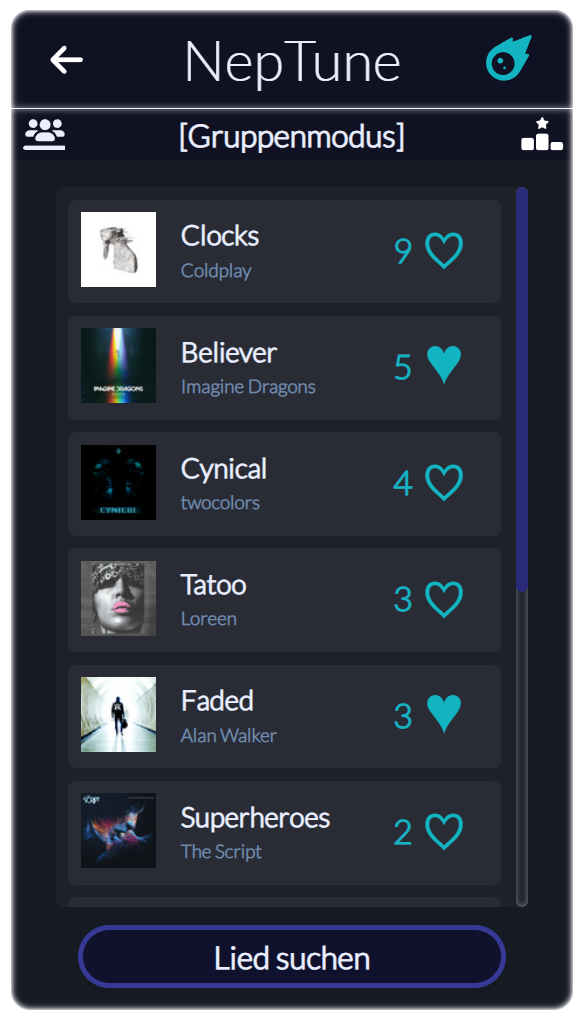
\includegraphics[width=0.4\textwidth]{LATEX/Pflichtenheft/GraphicDesigns/userVotePage.png}
    \captionof{figure}{sessionVoteView}
\end{center}

\textbf{<Button> Session-Info:}
\begin{itemize}
    \item <F 3.1> Durch Klicken auf den Button Session-Info (der mit dem Gruppen-Icon) gelangt man in die \hyperlink{sessionInfoView}{sessionInfoView}.
\end{itemize}

\textbf{<Textanzeige> Session-Modus:}
\begin{itemize}
    \item Zeigt den Modus der aktuellen Session an.
\end{itemize}

\textbf{<Button> Statistiken:}
\begin{itemize}
    \item <F 3.2> Durch Klicken auf den Button Statistiken (der mit dem Balken-Icon) gelangt man in die \hyperlink{sessionStatsView}{sessionStatsView}.
\end{itemize}

\textbf{<Track-Liste> Vorschlagsliste:}
\begin{itemize}
    \item Die Sammlung der angezeigten Tracks ist die Vorschlagsliste.
    \item <F 3.3.A> bzw. <F 3.3.B> beschreiben das Klicken auf den Upvote-Button, um einen Upvote hinzuzufügen bzw. zu entfernen.
\end{itemize}

\textbf{<Button> Track suchen:}
\begin{itemize}
    \item <F 3.4> Durch Klicken des Buttons ''Track suchen'' gelangt man in die \hyperlink{participantSearchView}{participantSearchView}.
\end{itemize}

\textbf{<Button> Zurück:}
\begin{itemize}
    \item <F 3.5> Beim Klicken des Zurück-Buttons erscheint ein Pop-Up Fenster mit der Frage ''Session wirklich verlassen?''. In diesem Pop-Up kann sich der Participant nun zwischen ''Ja'' und ''Nein'' entscheiden.
    \begin{itemize}
        \item <F 3.5.A> Durch Auswählen von ''Ja'' verlässt die Session und gelangt in die \hyperlink{startView}{startView}.
        \item <F 3.5.B> Durch Auswählen von ''Nein'' bleibt der Participant in der \hyperlink{sessionVoteView}{sessionVoteView}.
    \end{itemize}
\end{itemize}

\subsection{Tracksuche für Participants (participantSearchView)}
\label{sec:Benutzeroberfläche:participantSearchView}


\begin{center}
    \hypertarget{participantSearchView}{}
    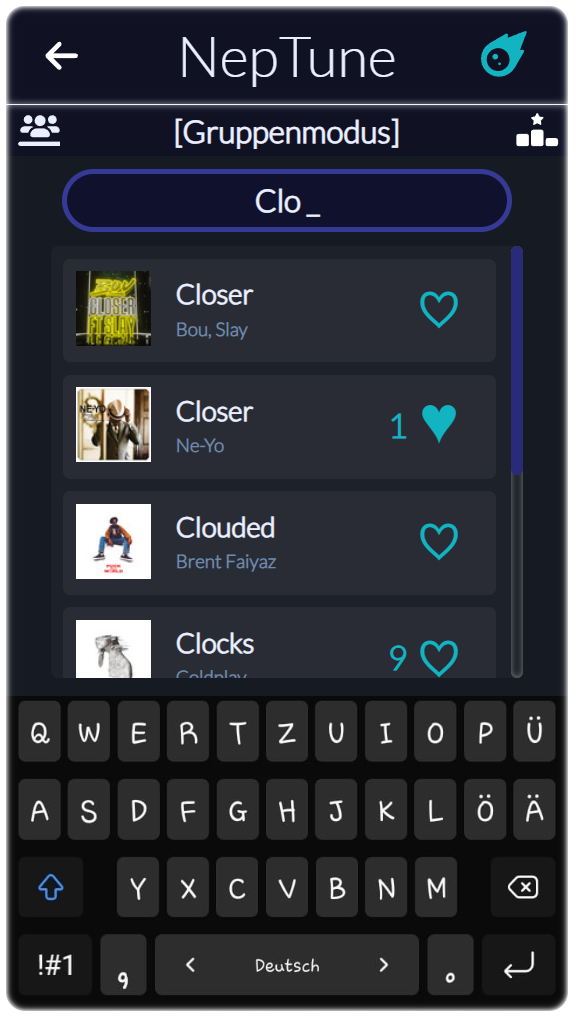
\includegraphics[width=0.4\textwidth]{LATEX/Pflichtenheft/GraphicDesigns/userSearchPage.png}
    \captionof{figure}{participantSearchView}
\end{center}

\textbf{<Button> Session-Info:}
\begin{itemize}
    \item <F 4.1> Durch Klicken auf den Button Session-Info (der mit dem Gruppen-Icon) gelangt man in die \hyperlink{sessionInfoView}{sessionInfoView}.
\end{itemize}

\textbf{<Textanzeige> Session-Modus:}
\begin{itemize}
    \item Zeigt den Modus der aktuellen Session an.
\end{itemize}

\textbf{<Button> Statistiken:}
\begin{itemize}
    \item <F 4.2> Durch Klicken auf den Button Statistiken (der mit dem Balken-Icon) gelangt man in die \hyperlink{sessionStatsView}{sessionStatsView}.
\end{itemize}

\textbf{<Eingabefeld> Track-Suchbegriff:}
\begin{itemize}
    \item Eingabefeld für den Eingabebegriff zur Suche nach Tracks.
    \item <F 4.3> Ändert sich der Eingabebegriff, werden die Track-Suchergebnisse aktualisiert.
    \item Die Tastatur wird standardmäßig beim Wechsel in die \hyperlink{participantSearchView}{participantSearchView} geöffnet.
\end{itemize}

\textbf{<Track-Liste> Track-Suchergebnisse:}
\begin{itemize}
    \item Die Sammlung der angezeigten Tracks ist bei Full Participants der gesamte Musikkatalog von Spotify, mit den zum Suchbegriff passenden Tracks. Dabei gelten folgende Einschränkungen:
    \begin{itemize}
        \item Im General Mode gibt es keine Einschränkungen.
        \item Im Artist Mode werden nur Tracks der vom Host bei \hyperlink{hostModeSettingsView}{Sessionerstellung} definierten Artists angezeigt.
        \item Im Genre Mode werden nur Tracks der vom Host bei \hyperlink{hostModeSettingsView}{Sessionerstellung} definierten Genres angezeigt.
        \item Im Playlist Mode werden nur Tracks der vom Host bei \hyperlink{hostModeSettingsView}{Sessionerstellung} definierten Playlist angezeigt.
    \end{itemize}
    \item Die Sammlung der angezeigten Tracks ist bei Restricted Participants nur die Vorschlagsliste.
    \item <F 4.4.A> bzw. <F 4.4.B> beschreiben das Klicken auf den Upvote-Button, um einen Upvote hinzuzufügen bzw. zu entfernen.
\end{itemize}

\textbf{<Button> Zurück:}
\begin{itemize}
    \item <F 4.5> Durch Klicken des Zurück-Buttons gelangt man in die  \hyperlink{sessionVoteView}{sessionVoteView}.
\end{itemize}


\subsection{Moduswahl für den Host (hostModeSelectView)}
\label{sec:Benutzeroberfläche:hostModeSelectView}


\begin{center}
    \hypertarget{hostModeSelectView}{}
    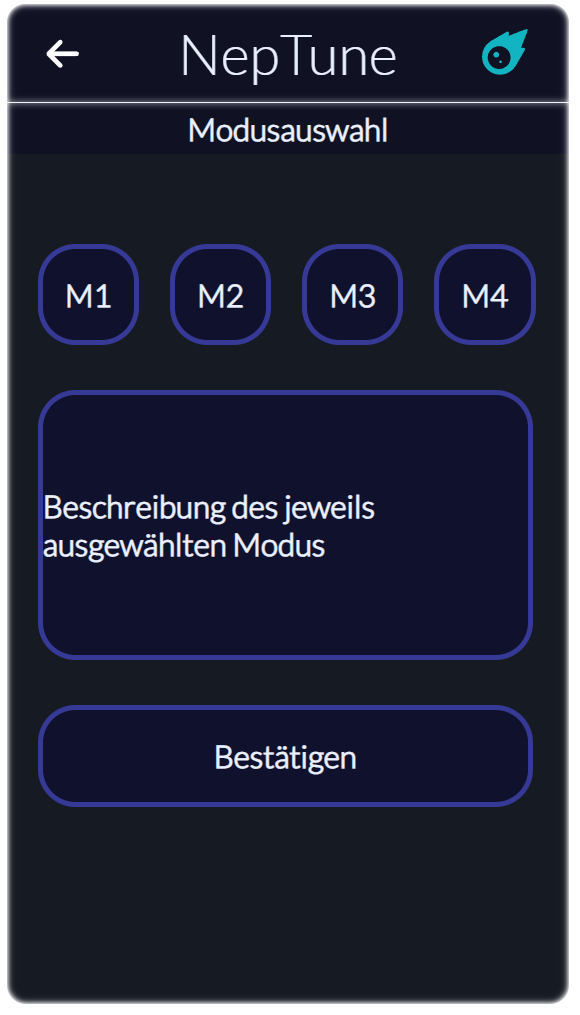
\includegraphics[width=0.4\textwidth]{LATEX/Pflichtenheft/GraphicDesigns/hostModusSelectPage.png}
    \captionof{figure}{hostModeSelectView}
\end{center}

\textbf{<Buttons> Modus-Buttons:}
\begin{itemize}
    \item Es stehen vier Modus-Buttons zur Verfügung:
    \begin{itemize}
        \item Der erste Button ist für den General Mode \hyperlink{GeneralMode}{(Use-Case-Diagramm)}
        \item Der zweite Button ist für den Artist Mode \hyperlink{Artist Mode}{(Use-Case-Diagramm)}
        \item Der dritte Button ist für den Genre Mode \hyperlink{Genre Mode}{(Use-Case-Diagramm)}
        \item Der vierte Button ist für den Playlist Mode \hyperlink{Playlist Mode}{(Use-Case-Diagramm)}
    \end{itemize}
    \item <F 5.1.A/B/C/D> Durch Klicken auf einen der vier Modus-Buttons wird dieser markiert. Es kann stets nur ein Modus-Button markiert sein. Zu Beginn ist der erste Button markiert. Der Modus des markierten Buttons ist angewählt.
\end{itemize}

\textbf{<Textanzeige> Modus-Info-Anzeige:}
\begin{itemize}
    \item Die Anzeige beinhaltet eine kurze Beschreibung des angewählten Modus.
\end{itemize}

\textbf{<Button> Bestätigen:}
\begin{itemize}
    \item <F 5.2> Durch Klicken des Bestätigen-Buttons wird der angewählte Modus übernommen und der Host gelangt in die \hyperlink{hostModeSettingsView}{hostModeSettingsView}.
\end{itemize}

\textbf{<Button> Zurück:}
\begin{itemize}
    \item <F 5.3> Durch Klicken des Zurück-Buttons gelangt man in die  \hyperlink{startView}{startView}.
\end{itemize}



\subsection{Moduseinstellungen für den Host (hostModeSettingsView)}
\label{sec:Benutzeroberfläche:hostModeSettingsView}

\begin{center}
    \hypertarget{hostModeSettingsView}{}
    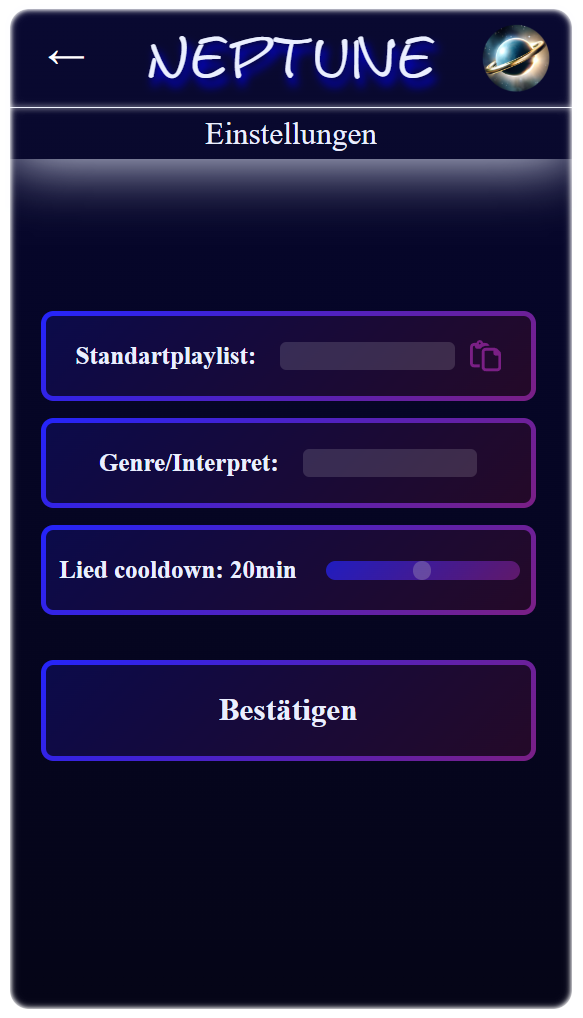
\includegraphics[width=0.4\textwidth]{LATEX/Pflichtenheft/GraphicDesigns/hostModusSettingsPage.png}
    \captionof{figure}{hostModeSettingsView}
\end{center}

\textbf{<Eingabefeld> Playlist-Link:}
\begin{itemize}
    \item <F 6.1> Eingabefeld zum Einfügen eines gültigen Spotify-Share-Links der gewünschten Playlist.
    \item Dieses Feld muss im Playlistmodus gefüllt werden, darf aber auch in jedem anderen Modus benutzt werden. Wurde eine Playlist in einem anderem Modus als dem Playlist-Mode eingegeben, dient diese als Quelle für weitere Tracks der Queue, falls die Queue leer ist und sich keine Tracks mehr in der Vorschlagsliste befinden.
\end{itemize}

\textbf{<Button> Artist-Auswahl:}
\begin{itemize}
    \item Nur im Artsit Mode vorhanden.
    \item <F 6.2> Durch Klicken der Artist-Auswahl gelangt man in die  \hyperlink{artistSelectView}{artistSelectView}.
\end{itemize}

\textbf{<Button> Genre-Auswahl:}
\begin{itemize}
    \item Nur im Genre Mode vorhanden.
    \item <F 6.3> Durch Klicken der Genre-Auswahl gelangt man in die  \hyperlink{genreSelectView}{genreSelectView}.
\end{itemize}

\textbf{<Slider> Track-Cooldown:}
\begin{itemize}
    \item <F 6.4> In jedem Modus vorhanden: Ein Slider zur Auswahl des zeitlichen Cooldowns bis ein gespielter Track erneut zum Upvoten verfügbar wird.
    \item Der derzeit eingestellte Wert wird neben dem Slider angezeigt.
    \item Der Wertebereich des Sliders geht von 0 Minuten bis 12 Stunden und verläuft nicht linear, sondern eher aber möglicherweise nicht exakt exponentiell.
\end{itemize}

\textbf{<Button> Bestätigen:}
\begin{itemize}
    \item Der Bestätigen-Button ist zunächst verblasst und nicht klickbar. Er wird erst klickbar, nachdem je nach Modus eine Playlist, mindestens ein Artist oder mindestens ein Genre eingestellt wurden.
    \item <F 6.5> Durch Klicken des Bestätigen-Buttons werden die Einstellungen angewendet und die Session eröffnet. Der Host gelangt in die \hyperlink{hostControlView}{hostControlView}.
\end{itemize}

\textbf{<Button> Zurück:}
\begin{itemize}
    \item <F 6.6> Durch Klicken des Zurück-Buttons gelangt man in die  \hyperlink{hostModeSelectView}{hostModeSelectView}.
\end{itemize}



\subsection{Kontrollansicht für den Host (hostControlView)}
\label{sec:Benutzeroberfläche:hostControlView}

\begin{center}
    \hypertarget{hostControlView}{}
    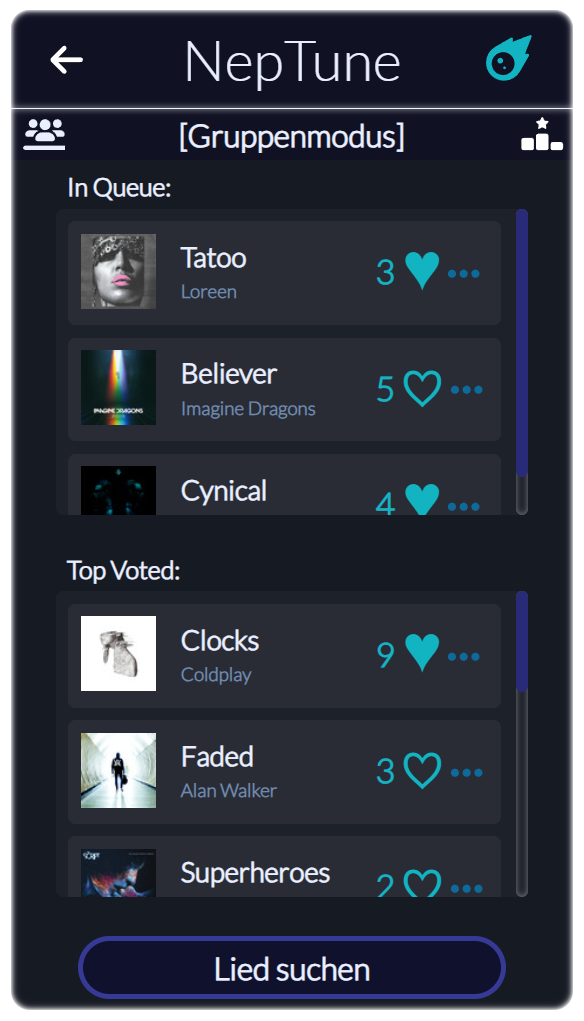
\includegraphics[width=0.4\textwidth]{LATEX/Pflichtenheft/GraphicDesigns/hostControlPage.png}
    \captionof{figure}{hostControlView}
\end{center}

\textbf{<Button> Session-Info:}
\begin{itemize}
    \item <F 7.1> Durch Klicken auf den Button Session-Info (der mit dem Gruppen-Icon) gelangt man in die \hyperlink{sessionInfoView}{sessionInfoView}.
\end{itemize}

\textbf{<Textanzeige> Session-Modus:}
\begin{itemize}
    \item Zeigt den Modus der aktuellen Session an.
\end{itemize}

\textbf{<Button> Statistiken:}
\begin{itemize}
    \item <F 7.2> Durch Klicken auf den Button Statistiken (der mit dem Balken-Icon) gelangt man in die \hyperlink{sessionStatsView}{sessionStatsView}.
\end{itemize}

\textbf{<Track-Liste> Queue-Anzeige:}
\begin{itemize}
    \item Die Sammlung der angezeigten Tracks ist die Queue.
    \item <F 7.3.A> bzw. <F 7.3.B> beschreiben das Klicken auf den Upvote-Button, um einen Upvote hinzuzufügen bzw. zu entfernen.
    \item <F 7.4> Der Track-Menü-Button bietet folgende Auswahlmöglichkeiten:
    \begin{itemize}
        \item <F 7.4.A> Track aus Queue entfernen
        \item <F 7.4.B> Track sperren
    \end{itemize}
    \item <F 7.5> Jeder Track lässt sich per Drag-and-Drop innerhalb der Queue-Anzeige verschieben, um die Reihenfolge anzupassen. Ein Ziehen auf die Vorschlagsliste entfernt ihn aus der Queue.
\end{itemize}

\textbf{<Track-Liste> Vorschlagsliste:}
\begin{itemize}
    \item Die Sammlung der angezeigten Tracks ist die Vorschlagsliste.
    \item <F 7.6.A> bzw. <F 7.6.B> beschreiben das Klicken auf den Upvote-Button, um einen Upvote hinzuzufügen bzw. zu entfernen.
    \item <F 7.7> Der Track-Menü-Button bietet folgende Auswahlmöglichkeiten:
    \begin{itemize}
        \item <F 7.7.A> Track unten zur Queue hinzufügen (Nur verfügbar, falls sich der Track noch nicht in der Queue befindet)
        \item <F 7.7.B> Track sperren
    \end{itemize}
    \item <F 7.8> Jeder Track lässt sich per Drag-and-Drop an eine bestimmte Stelle der Queue-Anzeige verschieben, um ihn an dieser Stelle in der Queue zu positionieren.
\end{itemize}

\textbf{<Button> Track suchen:}
\begin{itemize}
    \item <F 7.9> Durch Klicken des Buttons ''Track suchen'' gelangt man in die \hyperlink{hostSearchView}{hostSearchView}.
\end{itemize}

\textbf{Zurück-Button:}
\begin{itemize}
    \item <F 7.10> Beim Klicken des Zurück-Buttons erscheint ein Pop-Up Fenster mit der Frage ''Session wirklich löschen?''. In diesem Pop-Up kann sich der Host nun zwischen ''Ja'' und ''Nein'' entscheiden.
    \begin{itemize}
        \item <F 7.10.A> Durch Auswählen von ''Ja'' wird die Session gelöscht und der Host gelangt in die \hyperlink{startView}{startView}. Auch alle Participants der Session gelangen in die \hyperlink{startView}{startView}.
        \item <F 7.10.B> Durch Auswählen von ''Nein'' bleibt der Host in der \hyperlink{hostControlView}{hostControlView}.
    \end{itemize}
\end{itemize}

\subsection{Tracksuche für den Host (hostSearchView)}
\label{sec:Benutzeroberfläche:hostSearchView}


\begin{center}
    \hypertarget{hostSearchView}{}
    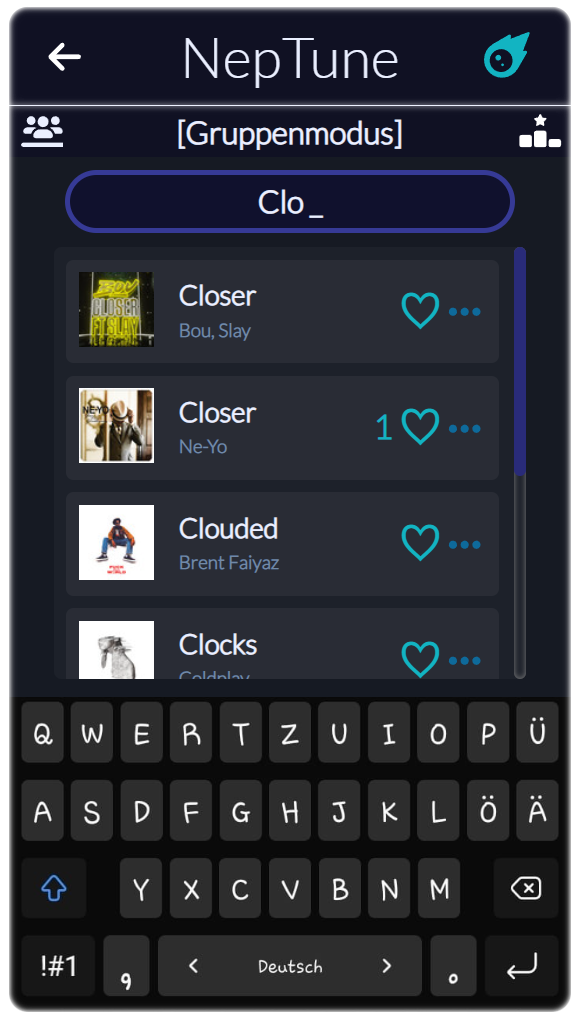
\includegraphics[width=0.4\textwidth]{LATEX/Pflichtenheft/GraphicDesigns/hostSearchPage.png}
    \captionof{figure}{hostSearchView}
\end{center}

Die hostSearchView ist identisch zur \hyperlink{participantSearchView}{participantSearchView}, die Testfälle seien hier mit <F 8.x> als F-Nummern versehen. Ausnahmen sind folgende Elementen, die anders definiert sind bzw. zusätzlich vorhanden sind:

\textbf{<Track-Liste> Track-Suchergebnisse:}
\begin{itemize}
    \item Die Sammlung der angezeigten Tracks ist gesamte Musikkatalog von Spotify, mit den zum Suchbegriff passenden Tracks. Dabei gelten ebenjene Einschränkungen aus der \hyperlink{participantSearchView}{participantSearchView}.
    \item <F 8.4.A> bzw. <F 8.4.B> beschreiben das Klicken auf den Upvote-Button, um einen Upvote hinzuzufügen bzw. zu entfernen.
    \item <F 8.5> Der Track-Menü-Button bietet folgende Auswahlmöglichkeiten:
    \begin{itemize}
        \item <F 8.5.A> Track hinten in die Queue hinzufpgen (Nur möglich, falls der Track noch nicht in der Queue ist)
        \item <F 8.5.B> Track sperren bzw. entsperren (Je nachdem ob der Track gesperrt bzw. entsperrt ist)
        \item <F 8.5.C> Cooldown aufheben (Nur möglich, falls der Track einen Cooldown besitzt)
    \end{itemize}
\end{itemize}

\textbf{<Button> Zurück:}
\begin{itemize}
    \item <F 8.6> Durch Klicken des Zurück-Buttons gelangt man in die  \hyperlink{hostControlView}{hostControlView}.
\end{itemize}

\textbf{<Button> Track-Filter:}
\begin{itemize}
    \item <F 8.7> Bei Anklicken des Track-Filter-Buttons (der mit dem Filter-Icon) öffnet sich ein kleines Dropdown-Menü mit zwei Auswahlmöglichkeiten zur Filter-Aktivierung:
    \begin{itemize}
        \item <F 8.7.A> Dem Cooldown-Filter für Tracks mit Cooldown (Filter-Icon mit kleiner Uhr)
        \item <F 8.7.B> Dem Sperr-Filter für gesperrte Tracks (Filter-Icon mit kleinem Schloss)
    \end{itemize}
    \item Durch Aktivieren werden in der Track-Anzeige nur Tracks angezeigt, welche auf den Filter zutreffen.
    \item Das angezeigte Filter-Icon ist das des aktiven Filters.
    \item <F 8.7.C> Wird das bereits aktive Filter-Icon erneut angeklickt, so wird der Filter deaktiviert.
    \item Es kann stets nur ein Filter aktiv sein.
\end{itemize}


\subsection{Session-Info (sessionInfoView)}
\label{sec:Benutzeroberfläche:sessionInfoView}

\begin{center}
    \hypertarget{sessionInfoView}{}
    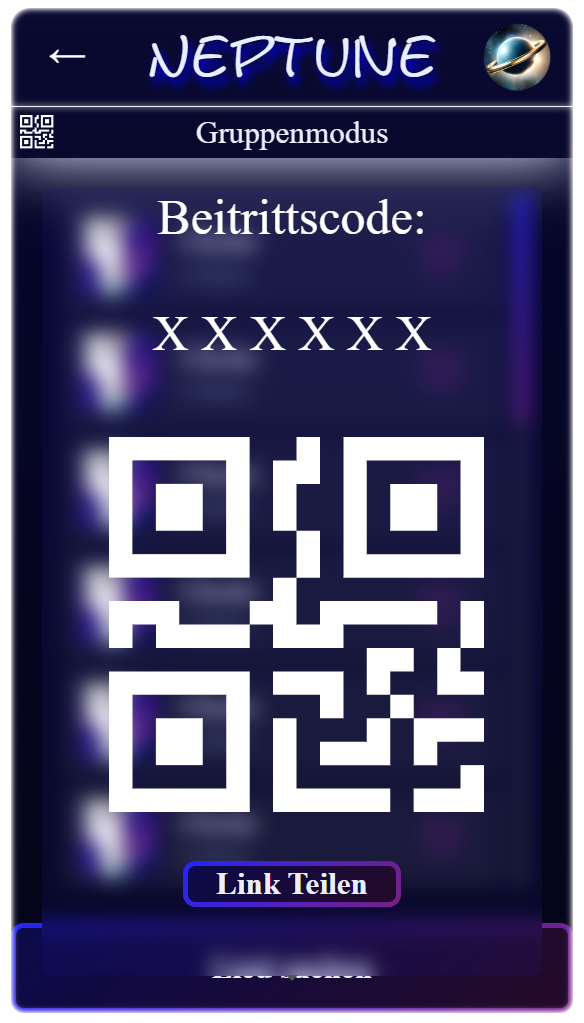
\includegraphics[width=0.4\textwidth]{LATEX/Pflichtenheft/GraphicDesigns/shareLinkPopUpPage.png}
    \captionof{figure}{sessionInfoView}
\end{center}

\textbf{<Anzeige> Sessionmodus:}
\begin{itemize}
    \item Anzeige des aktuellen Modus der Session.
\end{itemize}

\textbf{<Anzeige> Artist/Genre-Info:}
\begin{itemize}
    \item Nur im Artist oder Genre Mode: Anzeige der erlaubten Artists oder Genres.
\end{itemize}

\textbf{<Anzeige> Beitrittscode:}
\begin{itemize}
    \item Anzeige des sechsstelligen Codes zum Beitritt der Session.
\end{itemize}

\textbf{<QR-Code-Anzeige> QR-Code:}
\begin{itemize}
    \item Scannbare Anzeige des sechsstelligen Codes zum Beitritt der Session als QR-Code.
\end{itemize}

\textbf{<Anzeige> Share-Link:}
\begin{itemize}
    \item Kopierbare Anzeige eines Links zum Beitreten der Session.
\end{itemize}

\textbf{<Button> Link teilen:}
\begin{itemize}
    \item <F 9.1> Teilt beim Klicken den Link zum Beitreten der Session über die Android-Schnittstelle zum Teilen von Inhalten.
\end{itemize}

\textbf{<Button> Zurück:}
\begin{itemize}
    \item <F 9.2> Durch Klicken des Zurück-Buttons gelangt man in die letzte View auf dem Backstack, von der aus die sessionInfoView geöffnet wurde.
    \item (Es wird keinen X-Button geben, obwohl dieser im Grafikentwurf gezeigt wird.)
\end{itemize}


\subsection{Session-Statistiken (sessionStatsView)}
\label{sec:Benutzeroberfläche:sessionStatsView}


\begin{center}
    \hypertarget{sessionStatsView}{}
    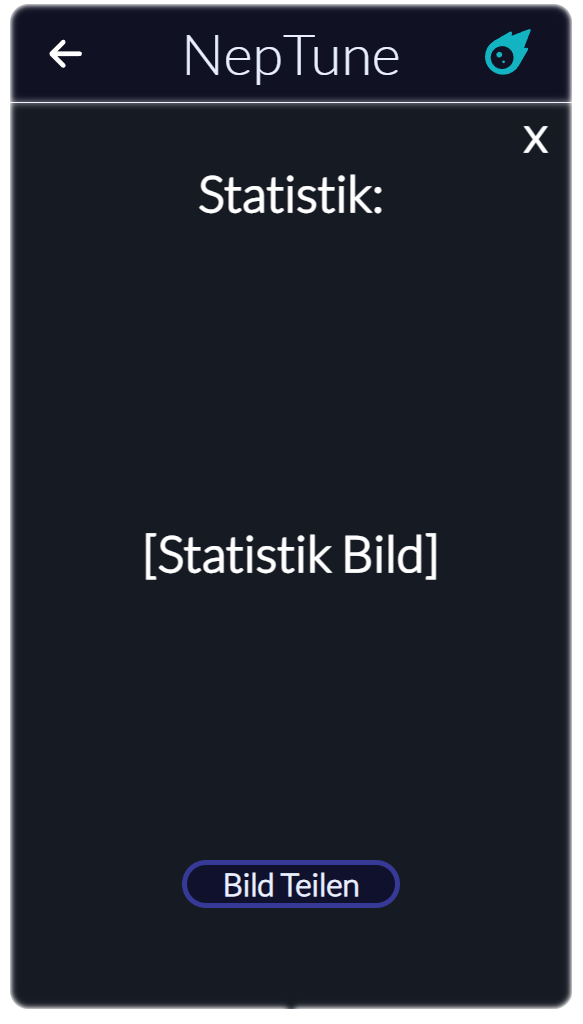
\includegraphics[width=0.4\textwidth]{LATEX/Pflichtenheft/GraphicDesigns/statisticsPopUpPage.png}
    \captionof{figure}{sessionStatsView}
\end{center}

\textbf{<Bild-Anzeige> Statistik-Bild:}
\begin{itemize}
    \item Anzeige eines generierten Bildes, das alle gewählten Statistiken über die Session aus den \hyperlink{Wunschkriterien}{Wunschkriterien} enthält.
\end{itemize}

\textbf{<Button> Statistik-Bild teilen:}
\begin{itemize}
    \item <F 10.1> Teilt beim Klicken das angezeigte Bild der Statistik über die Android-Schnittstelle zum Teilen von Inhalten.
\end{itemize}

\textbf{<Button> Zurück:}
\begin{itemize}
    \item <F 10.2> Durch Klicken des Zurück-Buttons gelangt man in die letzte View auf dem Backstack, von der aus die sessionInfoView geöffnet wurde.
    \item (Es wird keinen X-Button geben, obwohl dieser im Grafikentwurf gezeigt wird.)
\end{itemize}



\subsection{Artist-Auswahl (artistSelectView)}
\label{sec:Benutzeroberfläche:artistSelectView}

\hypertarget{artistSelectView}{}
TODO: AUSFÜLLEN


\subsection{Genre-Auswahl (genreSelectView)}
\label{sec:Benutzeroberfläche:genreSelectView}

\hypertarget{genreSelectView}{}
TODO: AUSFÜLLEN






\section{Weitere funktionale Anforderungen}
\label{sec:Benutzeroberfläche:Grafiken}

\begin{itemize}
    \item <F 100> Das vollständige Beenden der App wird durch das Verlassen der \hyperlink{startView}{startView} per Zurück-Button oder durch Android-System-Funktionalitäten ermöglicht.
    \item <F 101> Wenn die App vollständig beendet ist/war, öffnet sich beim Starten der App eine von drei Views:
    \begin{itemize}
        \item Die \hyperlink{userVoteView}{userVoteView} öffnet sich, wenn man derzeit Participant einer aktiven Session ist.
        \item Die \hyperlink{hostControlView}{hostControlView} öffnet sich, wenn man derzeit Host einer aktiven Session ist.
        \item Die \hyperlink{startView}{startView} öffnet sich, wenn man derzeit nicht Participant oder Host einer aktiven Session ist.
    \end{itemize}
    \item <F 102> Falls die App nicht vollständig beendet wurde und die Zustandsdaten des Android-Betriebssystems noch vorhanden sind, so öffnet sich die App in der Ansicht, in der man sie verlassen hat.
    \item Beim Beginn des tatsächlichen Abspielens wird der Track aus der Queue und der Vorschlagsliste entfernt. Die vorhandenen Upvotes werden auf null zurückgesetzt und der Track wird mit dem vom Host bei der \hyperlink{hostModeSettingsView}{Sessionerstellung} definierten Cooldown belegt.
    \item Eine Session kann entweder manuell durch den Host beendet werden, oder sie endet automatisch sobald: Die Queue leer ist und der derzeit abgespielte Song beendet ist. Sobald die Queue leer ist und der Host erreichbar ist (d.h. die App ausgeführt wird), wird nach den Regeln des Autoplays ein weiteres Lied in die Queue eingefügt. (TODO: WIRD DAS NOCH AKTUALISIERT; FALLS EIN ANDERES MEHR UPVOTES BEKOMMMT?)
    \item Die Anzeigesprache der App ist Deutsch, wenn Deutsch als Systemsprache des Geräts eingestellt ist. Falls eine andere Sprache als Systemsprache eingestellt ist, ist die Anzeigesprache der App Englisch.
    \item Die Verknüfung mit oder Trennung von Spotify wird dauerhaft gespeichert, auch nach vollständigem Beenden der App.
\end{itemize}

TODO: Am Ende der Session werden den Usern die Statistiken angezeigt. (WIE SETZEN WIR DAS UM???)






% show subsections in contents
\addtocontents{toc}{\protect\setcounter{tocdepth}{2}}
\chapter{Anwendungsfälle}
\label{chap:Anwendungsfälle}

In diesem Kapitel werden einige Anwendungsfälle der App mithilfe von Use Case Diagrammen anschaulich gemacht. Diese beschreiben das Starten einer Session, sowie die einzelnen Modi der App.

\section{Session erstellen}
\label{sec:Anwendungsfälle:Session erstellen}

\begin{figure}[h]
   \hypertarget{Anwendungsfaelle}{}
    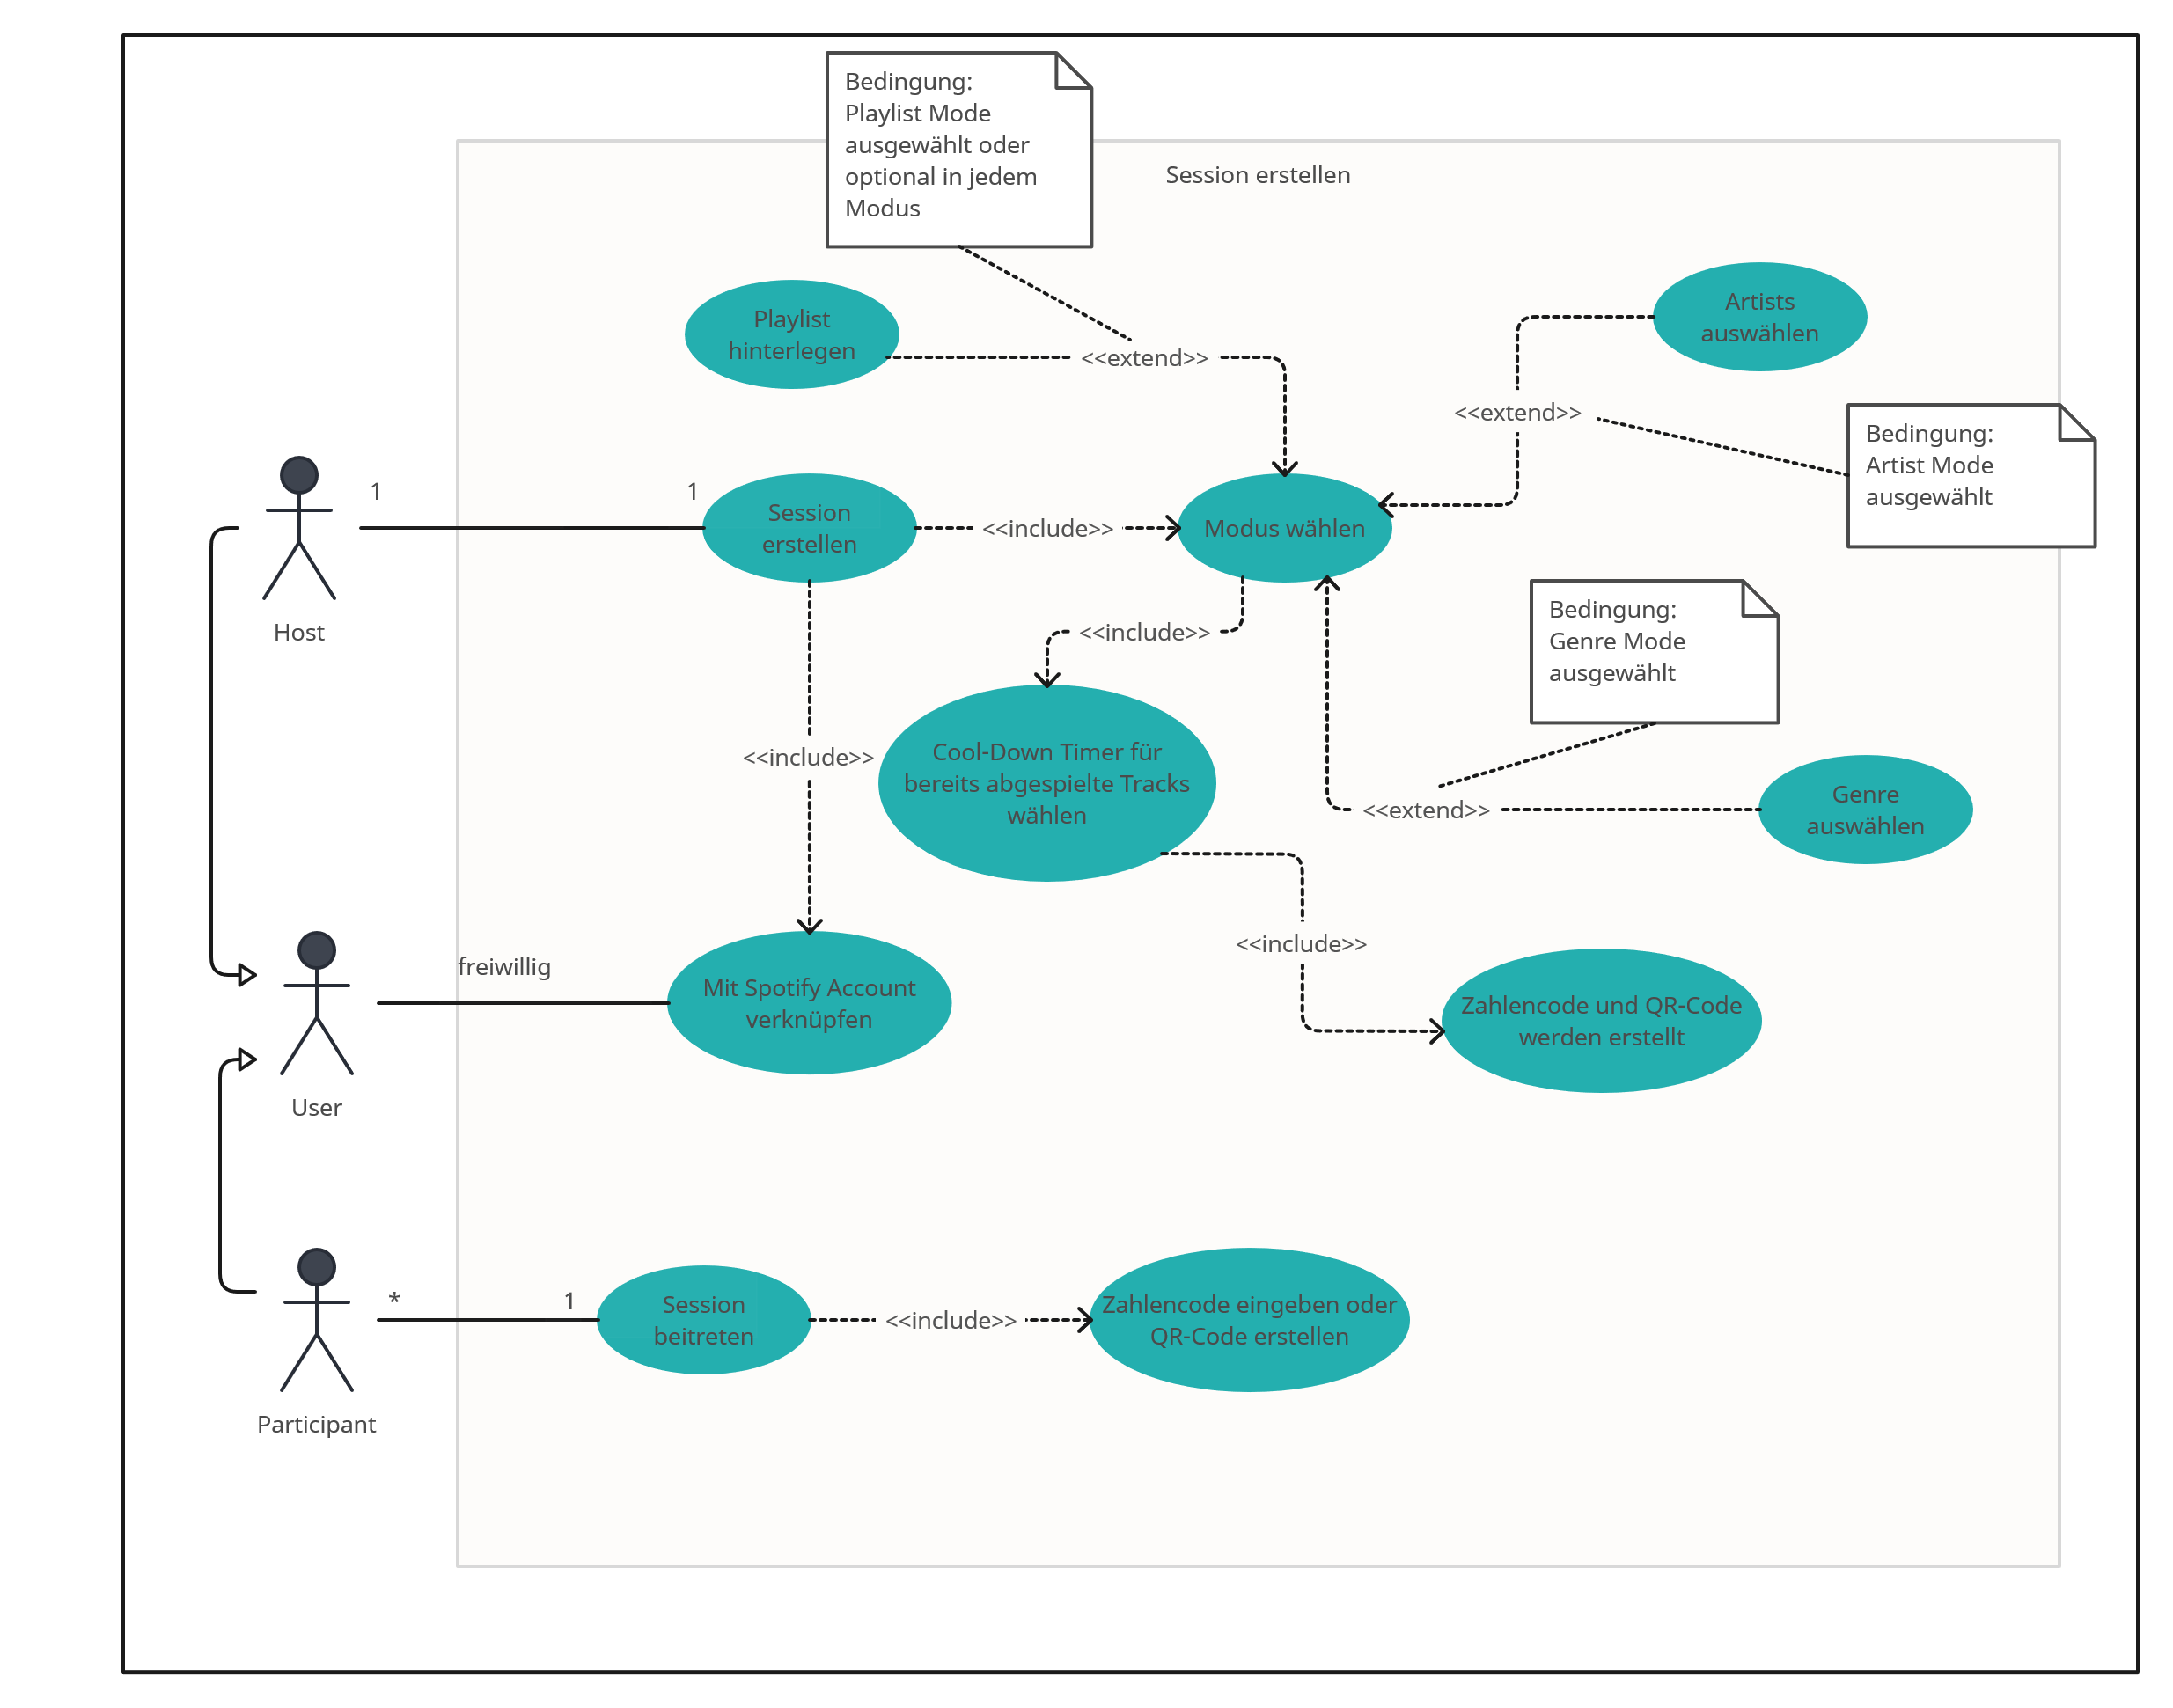
\includegraphics[width = 16cm]{LATEX/Pflichtenheft/GraphicDesigns/Use Case Session erstellen.png}
    \caption{Session erstellen}
    \label{fig:Use Case App Start}
\end{figure}

\newpage

\section{General Mode}
\label{sec:Anwendungsfälle:GeneralMode}

\begin{figure}[h]
    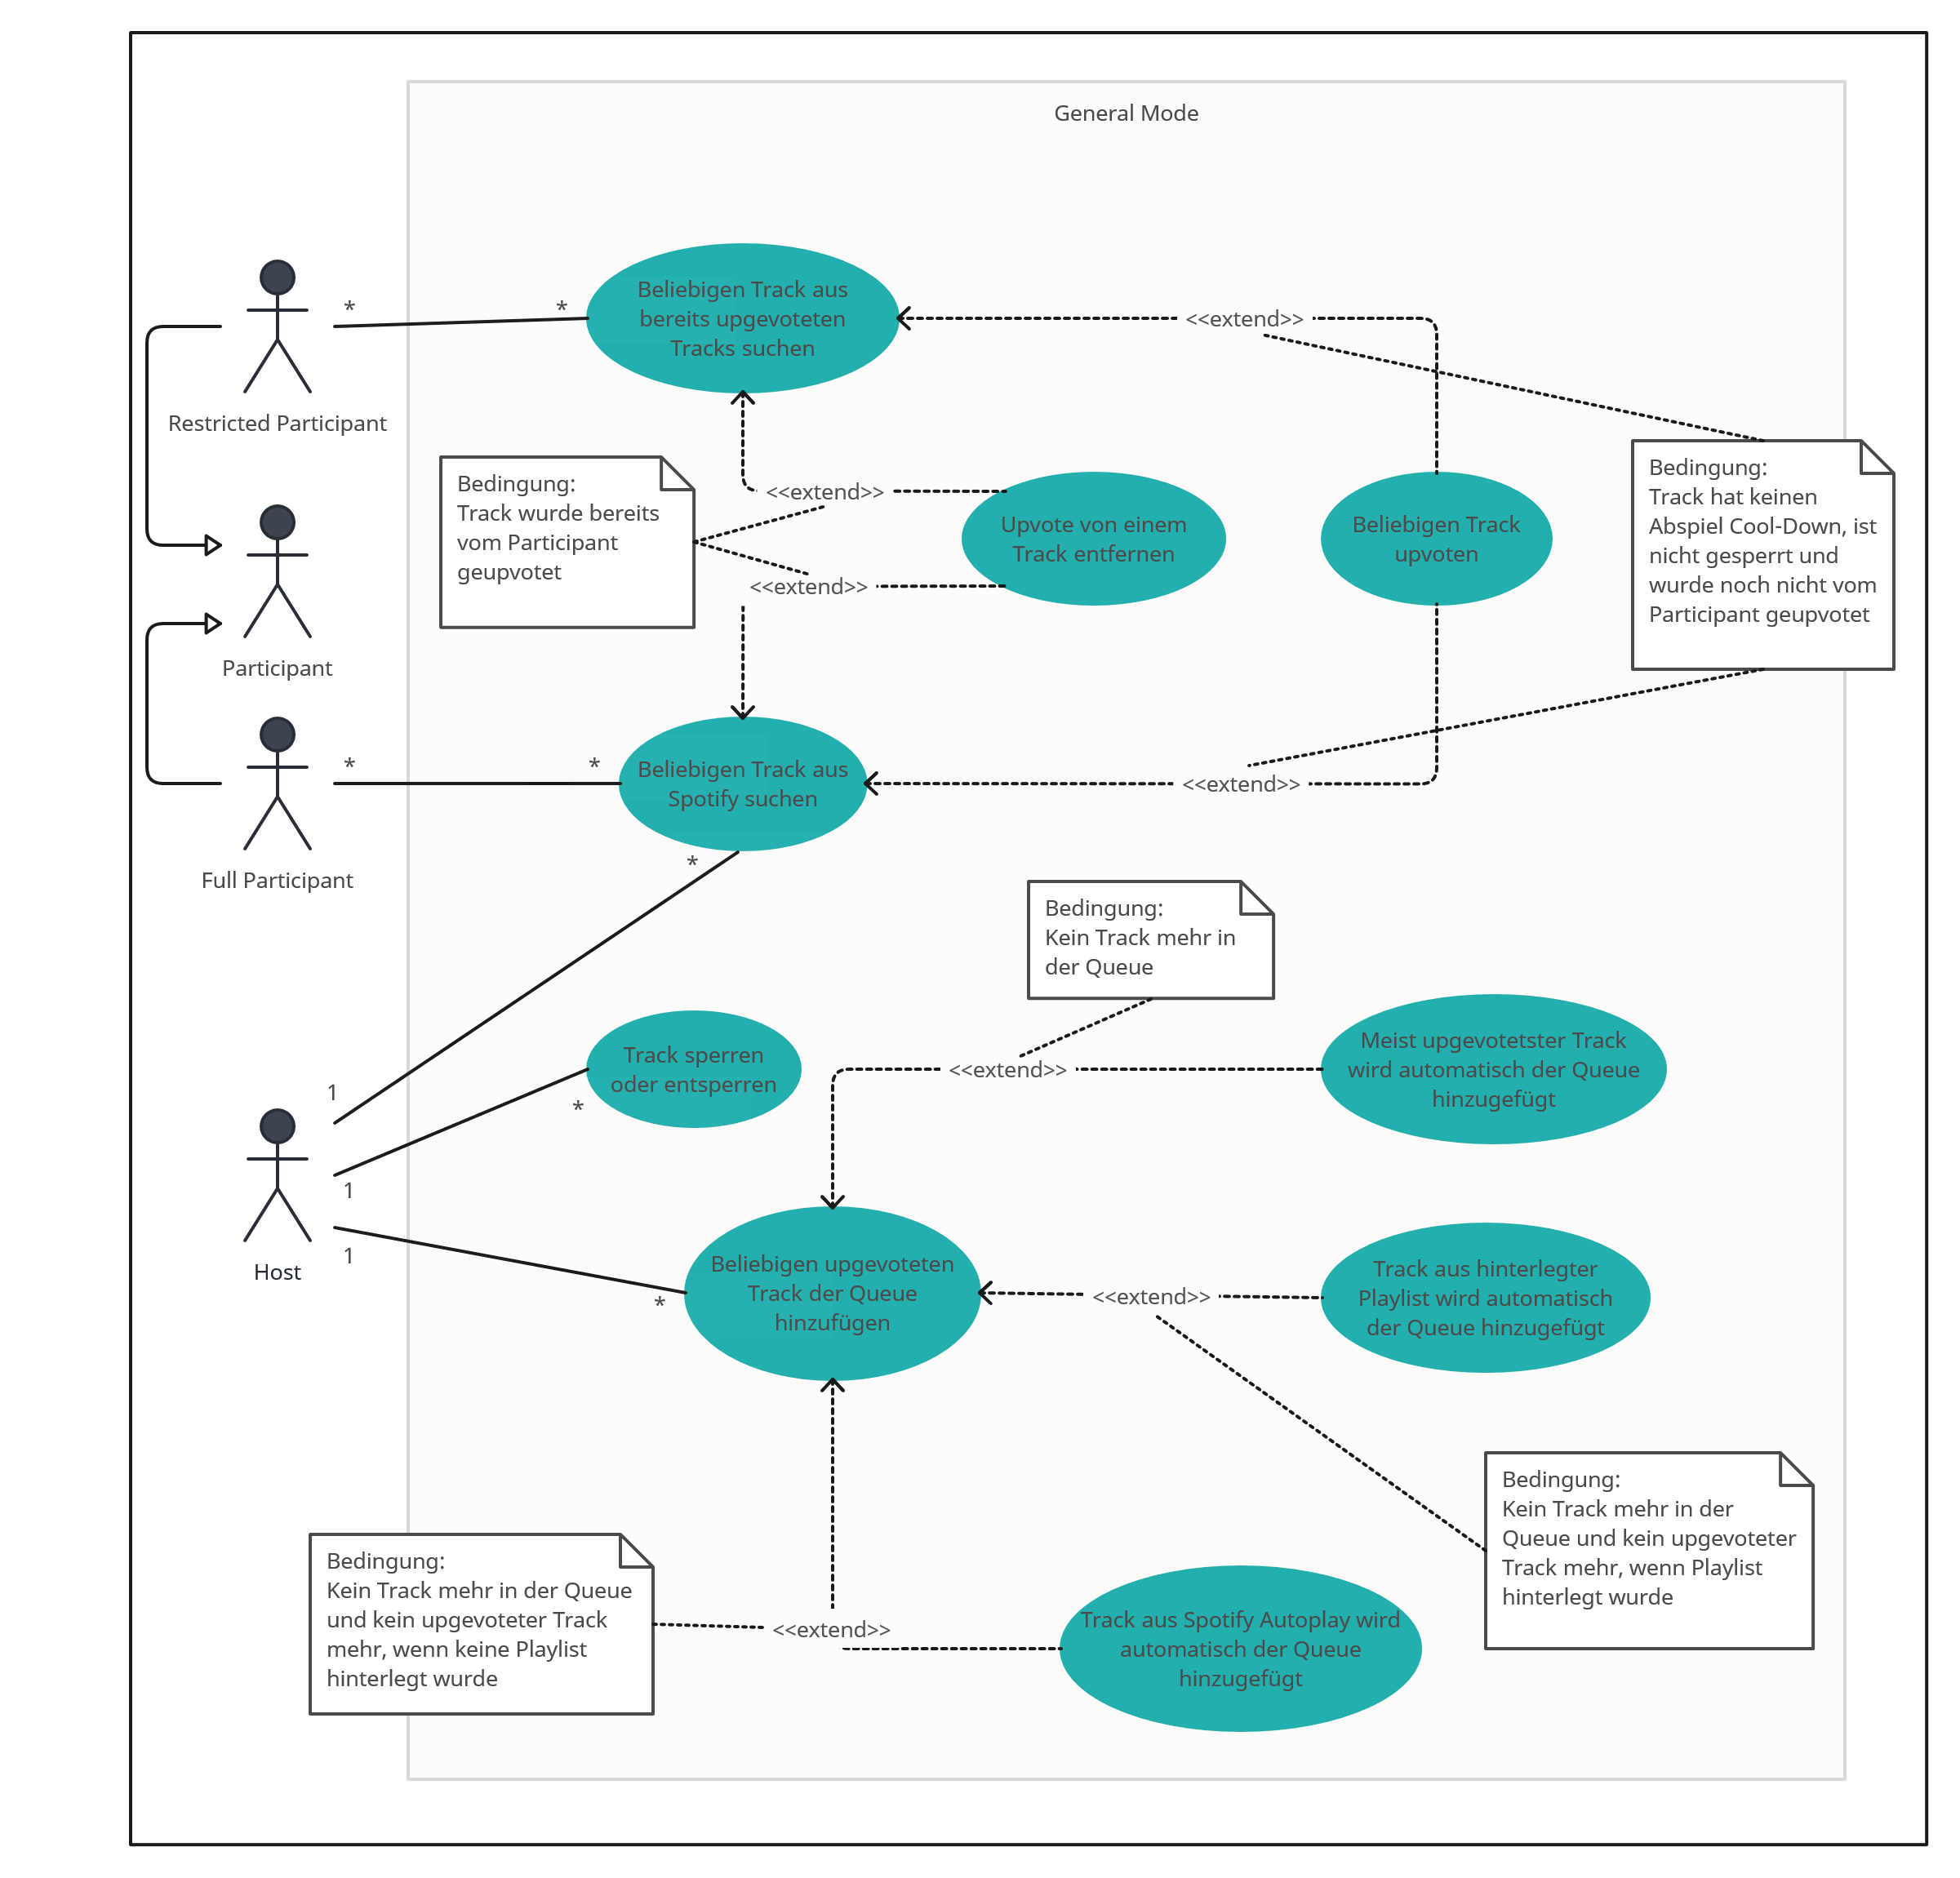
\includegraphics[width = 16cm]{LATEX/Pflichtenheft/GraphicDesigns/Use Case General Mode.png}
    \caption{General Mode}
    \label{fig:Use Case General Mode}
\end{figure}

\newpage

\section{Artist Mode}
\label{sec:Anwendungsfälle:Artist Mode}

\begin{figure}[h]
    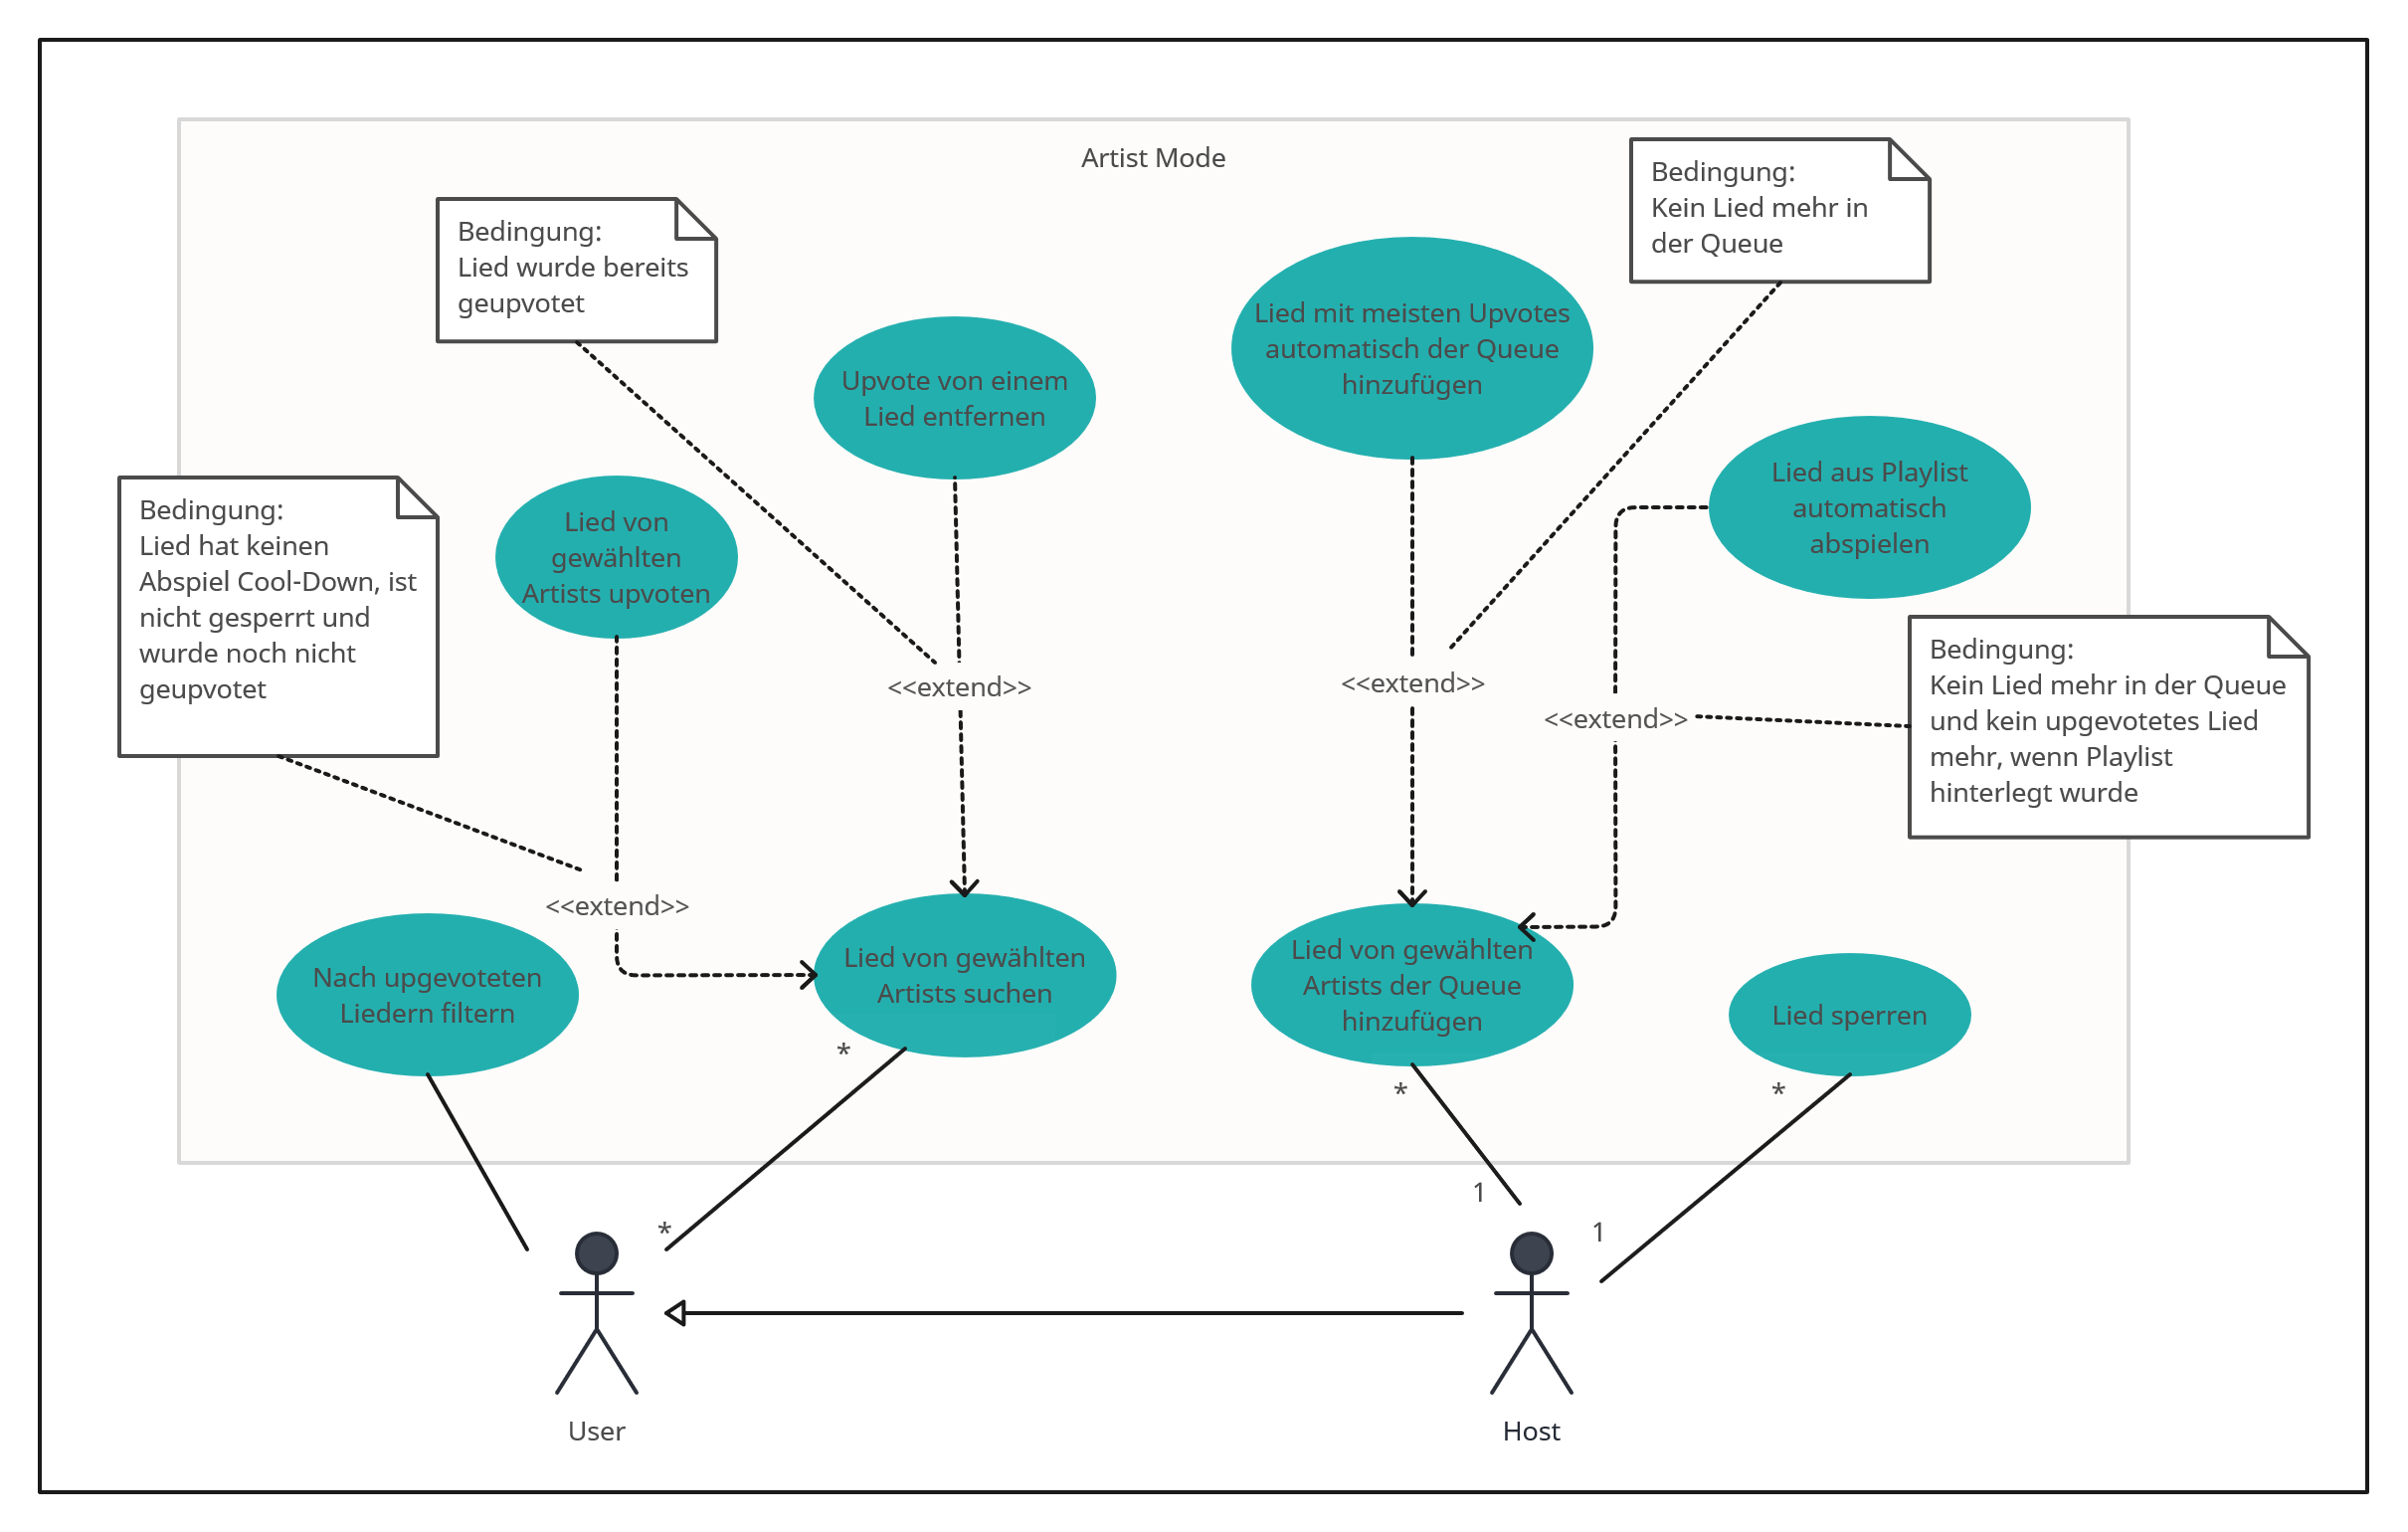
\includegraphics[width = 16cm]{LATEX/Pflichtenheft/GraphicDesigns/Use Case Artist Mode.png}
    \caption{Artist Mode}
    \label{fig:Use Case Artist Mode}
\end{figure}

\newpage

\section{Genre Mode}
\label{sec:Anwendungsfälle:Genre Mode}

\begin{figure}[h]
    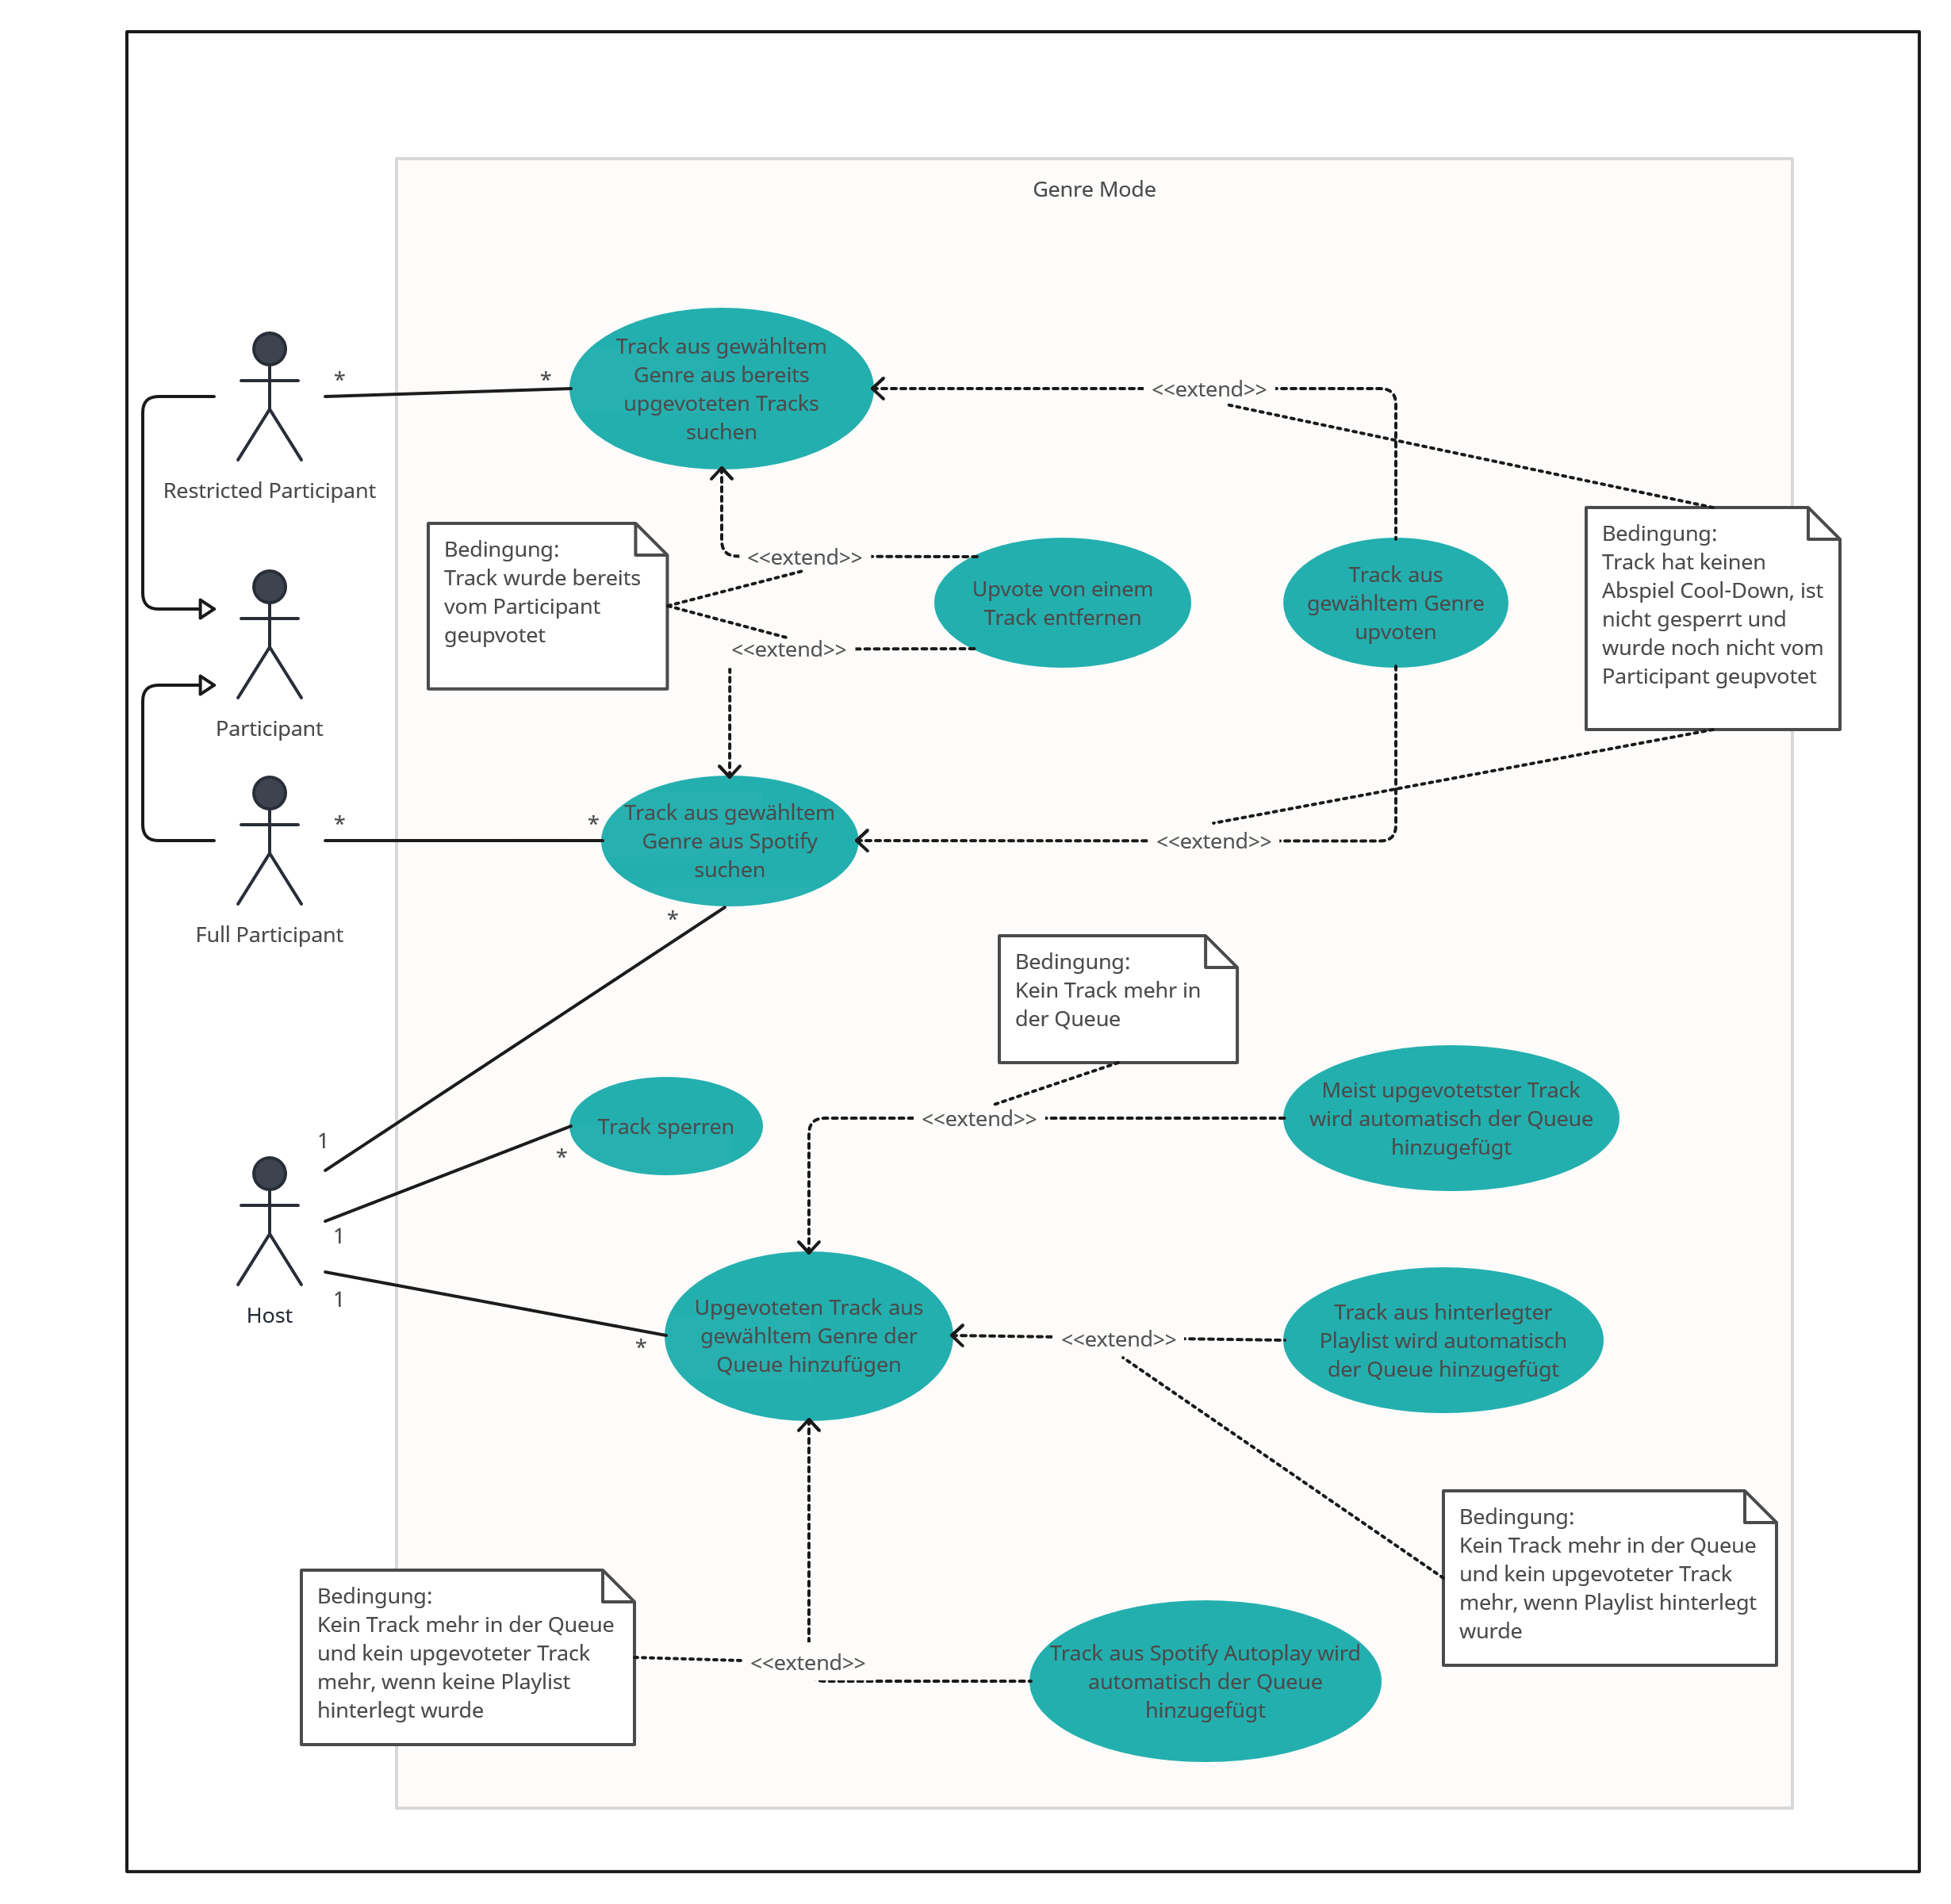
\includegraphics[width = 16cm]{LATEX/Pflichtenheft/GraphicDesigns/Use Case Genre Mode.png}
    \caption{Genre Mode}
    \label{fig:Use Case Genre Mode}
\end{figure}

\newpage

\section{Playlist Mode}
\label{sec:Anwendungsfälle:Playlist Mode}

\begin{figure}[h]
    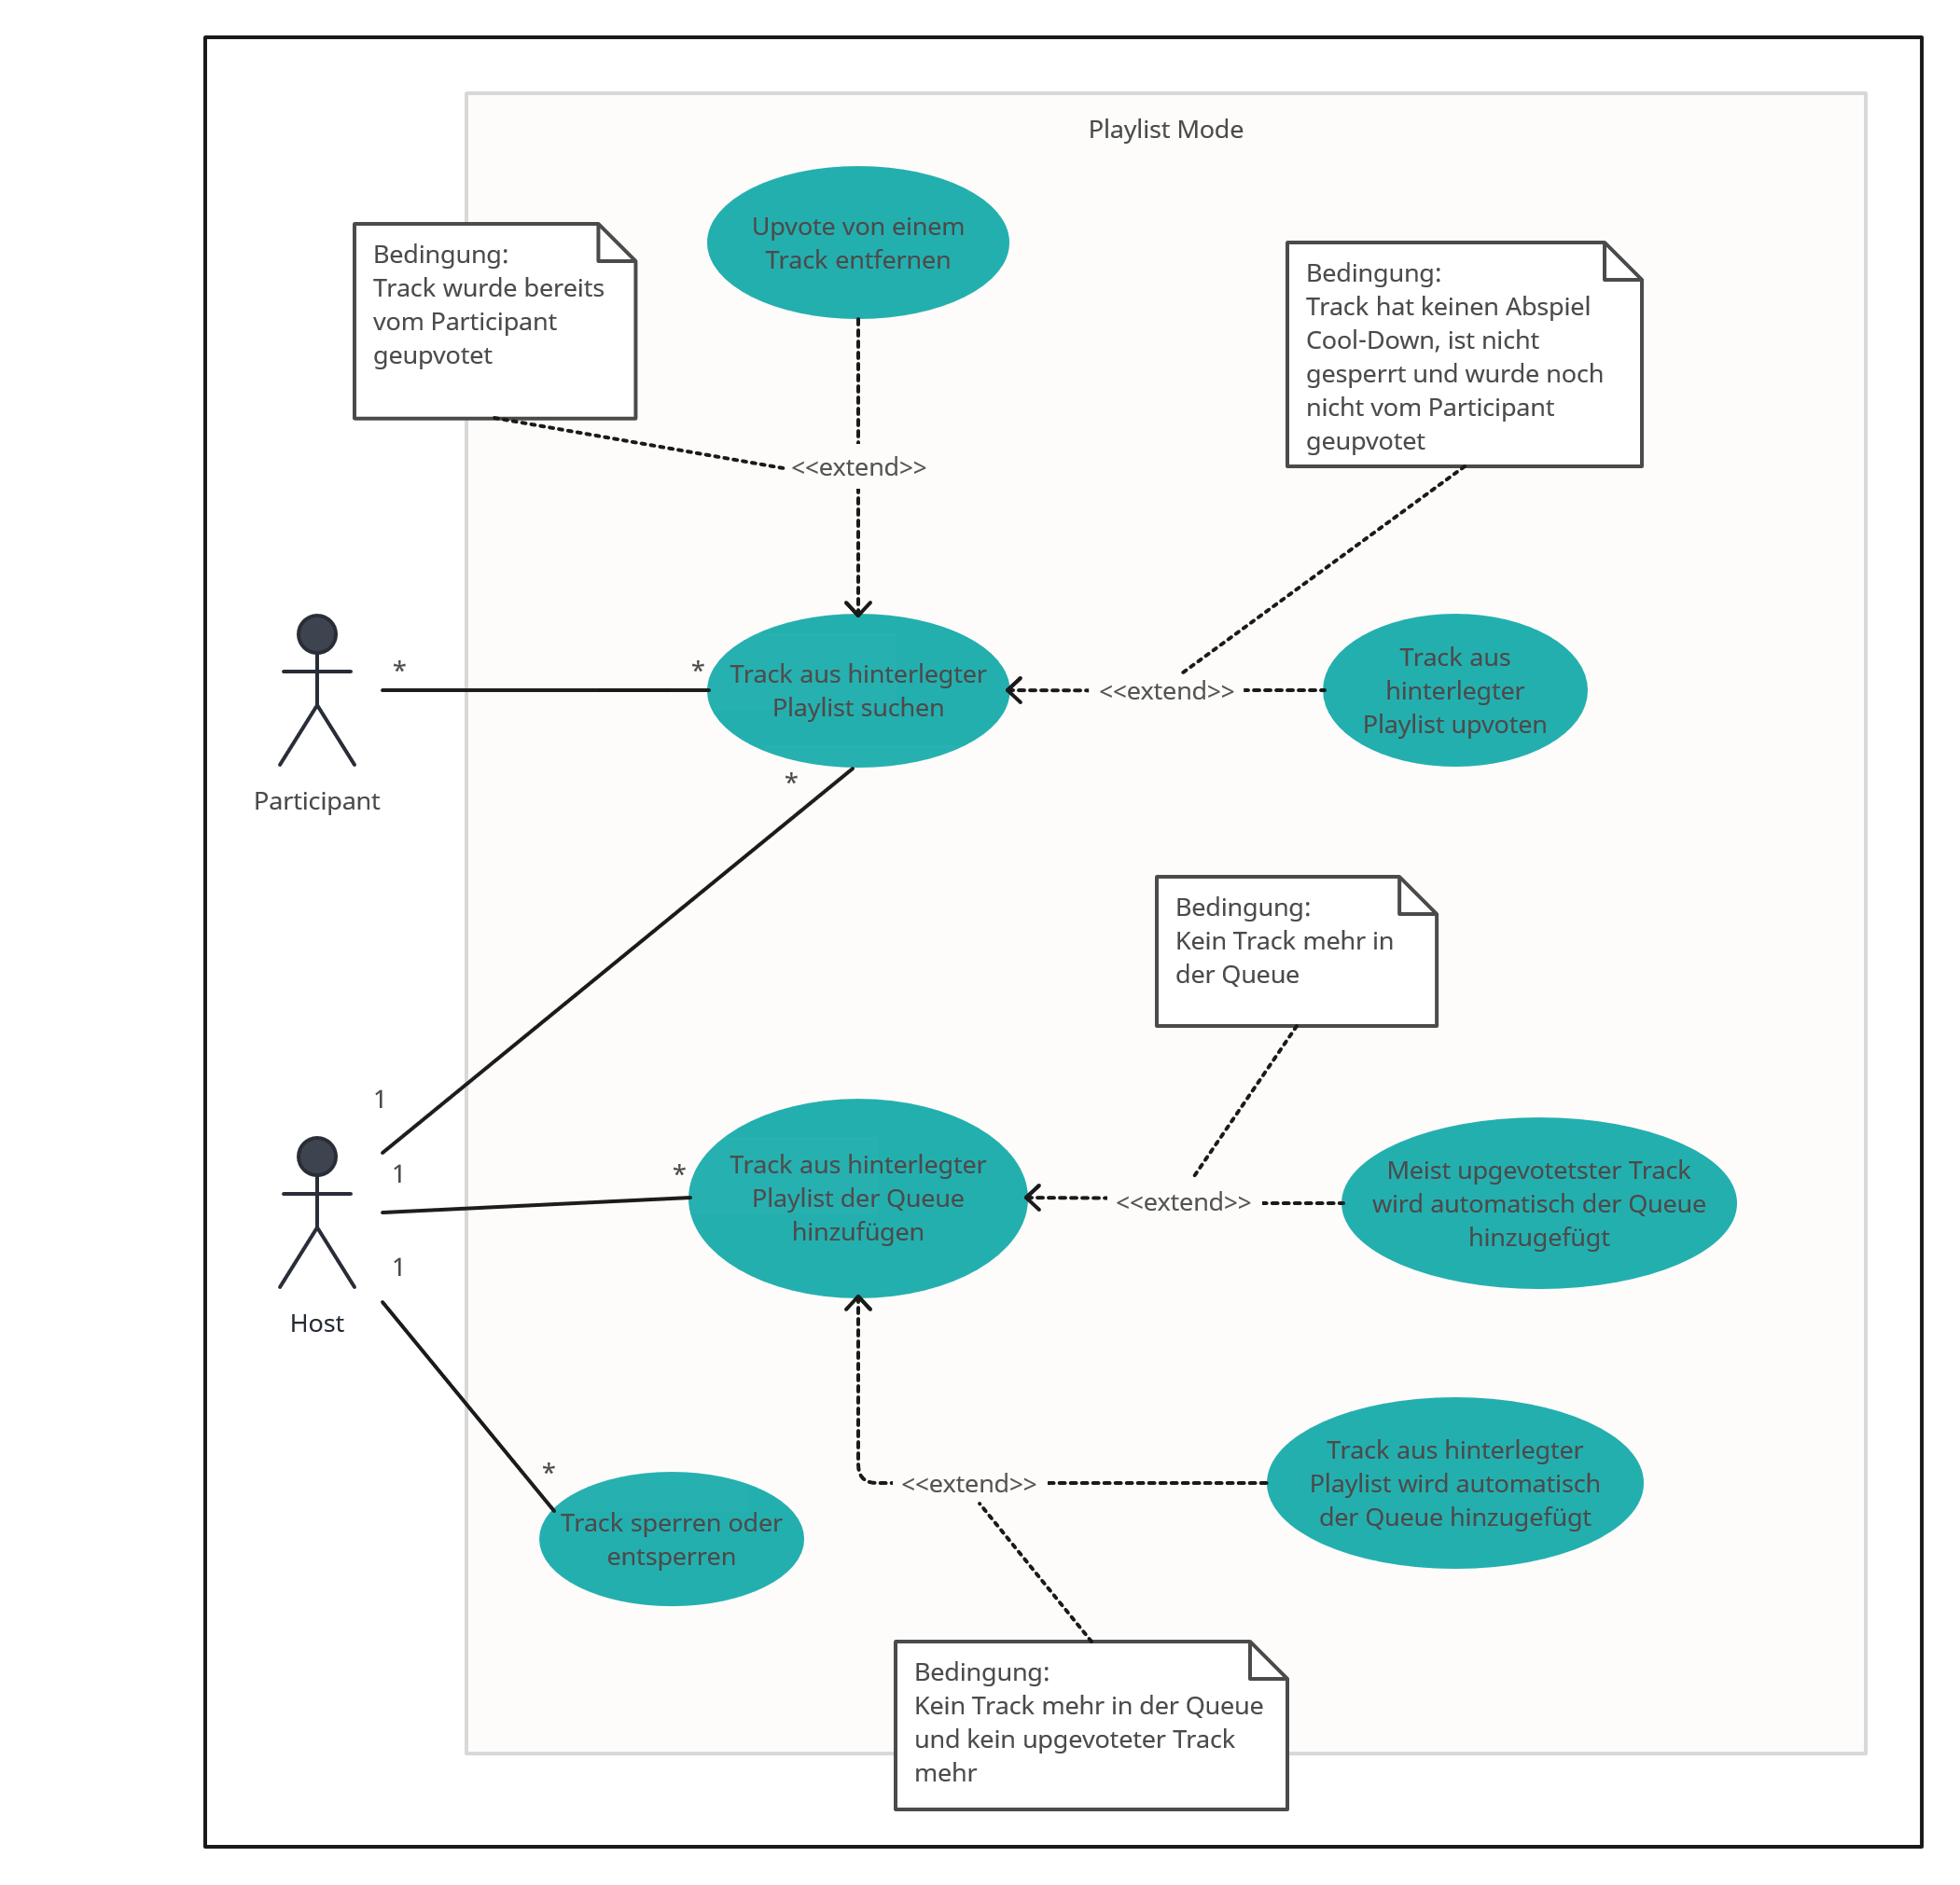
\includegraphics[width = 16cm]{LATEX/Pflichtenheft/GraphicDesigns/Use Case Playlist Mode.png}
    \caption{Playlist Mode}
    \label{fig:Use Case Playlist Mode}
\end{figure}



\chapter{Testfälle und -szenarien}
\label{chap:Tests}

In diesem Kapitel werden alle Testfälle und -szenarien definiert, die durch einen oder mehrere Benutzer des Produkts durchgeführt werden können. Dabei wird das definierte Verhalten erwartet- Die hier definierten Testfälle sollen explizit keine detaillierten technischen Funktionalitäten auf technischer Ebene testen. Die Überprüfung solcher detaillierten technischen Funktionalitäten wird durch Unittests abgedeckt, die während der Entwurfs- und Implementierungsphase entworfen und implementiert werden.

\section{Testfälle}
\label{sec:Tests:Testfälle}

Die Testfälle lassen sich den dem Kapitel Benutzeroberfläche und funktionale Anforderungen (Kapitel \ref{chap:Benutzeroberfläche}) entnehmen. Jede mit einer F-Nummer versehene funktionale Anforderung ist ein Testfall.

\section{Grundlegende Testszenarien}
\label{sec:Tests:GrundlegendeTestszenarien}
% do not show subsections in contents
\addtocontents{toc}{\protect\setcounter{tocdepth}{1}}

Grundlegende Testszenarien sind eine überschaubare und besonders essentielle Folge von Testfällen, die eine Benutzerinteraktion durchspielen. Sie setzen sich aus Testfällen oder bereits zuvor definierten grundlegenden Testszenarien zusammen.

\subsection{Grundlegendes Testszenario 1 (G1): Erstellen einer Session}
\label{subsec:Tests:GrundlegendeTestszenarien:G1}
Ein mit Spotify-Premium verknüpfter User erstellt eine Session mit einem bestimmten Modus M und wird so zu ihrem Host.
\begin{itemize}
    \item <F 101> Starten der App nach vollständiger Beendung
    \item <F 1.1> Beginnen der Sessionerstellung
    \item <F 5.1.M> Wahl des Modus
    \item <F 5.2> Bestätigen des Modus
    \item <F 6.1>, <F 6.2>/<F 6.3>, <F 6.4> Wählen entsprechender gültiger Einstellungen
    \item <F 6.5> Bestätigen und Beginn der Session
\end{itemize}


\subsection{Grundlegendes Testszenario 2 (G2): Beitritt einer Session als Full Participant}
\label{subsec:Tests:GrundlegendeTestszenarien:G2}
Ein User tritt als Full Participant einer Session mit einem bestimmten Modus bei, die von einem anderen User als Host erstellt wurde.
Dazu muss bereits G1 (\ref{subsec:Tests:GrundlegendeTestszenarien:G1}) abgelaufen sein.
\begin{itemize}
    \item <F 101> Starten der App nach vollständiger Beendung
    \item <F 1.1> Beginnen des Sessionbeitrittsvorgangs
    \item <F 2.1> Eingabe des Zugangscodes zum Sessionbeitritt
    \item <F 2.2.A> Bestätigung des Zugangscodes zum Sessionbeitritt
\end{itemize}


\subsection{Grundlegendes Testszenario 3 (G3): Beitritt einer Session als Restricted Participant}
\label{subsec:Tests:GrundlegendeTestszenarien:G3}
Ein User, tritt als Restricted Participant einer Session mit einem bestimmten Modus bei, die von einem anderen User als Host erstellt wurde.
Dazu muss bereits G1 (\ref{subsec:Tests:GrundlegendeTestszenarien:G1}) abgelaufen sein.
\begin{itemize}
    \item <F 101> Starten der App nach vollständiger Beendung
    \item <F 1.1> Beginnen des Sessionbeitrittsvorgangs
    \item <F 2.1> Eingabe des Zugangscodes zum Sessionbeitritt
    \item <F 2.2.A> Bestätigung des Zugangscodes zum Sessionbeitritt
\end{itemize}

\subsection{Grundlegendes Testszenario 4 (G4): Upvoten eines neuen Tracks als Full Participant}
\label{subsec:Tests:GrundlegendeTestszenarien:G4}
Ein User, der schon als Full Particpant einer Session mit einem bestimmten Modus beigetreten ist, die von einem anderen User als Host erstellt wurde, votet einen neuen Track up. \\
Dazu muss bereits G1 (\ref{subsec:Tests:GrundlegendeTestszenarien:G1}) und dann G2 (\ref{subsec:Tests:GrundlegendeTestszenarien:G2}) abgelaufen sein.
\begin{itemize}
    \item <F 3.4> Öffnen der Tracksuche
    \item <F 4.3> Suchen eines Tracks
    \item <F 4.4.A> Upvoten des Tracks
\end{itemize}

\subsection{Grundlegendes Testszenario 5 (G5): Upvoten eines neuen Tracks als Host}
\label{subsec:Tests:GrundlegendeTestszenarien:G5}
Der Host votet einen neuen Track up. \\
Dazu muss bereits G1 (\ref{subsec:Tests:GrundlegendeTestszenarien:G1}) abgelaufen sein.
\begin{itemize}
    \item <F 7.9> Öffnen der Tracksuche
    \item <F 8.3> Suchen eines Tracks
    \item <F 8.4.A> Upvoten des Tracks
\end{itemize}

\subsection{Grundlegendes Testszenario 6 (G6): Upvoten eines Songs}
\label{subsec:Tests:GrundlegendeTestszenarien:G6}
Ein Participant einer Session mit einem bestimmten Modus votet einen Track aus der Vorschlagsliste up. \\
Dazu muss bereits G1 (\ref{subsec:Tests:GrundlegendeTestszenarien:G1}) und dann G2 oder G3 (\ref{subsec:Tests:GrundlegendeTestszenarien:G2} oder \ref{subsec:Tests:GrundlegendeTestszenarien:G3}) und dann G4 (\ref{subsec:Tests:GrundlegendeTestszenarien:G4}) abgelaufen sein.
\begin{itemize}
    \item <F 3.3.A> Upvote für einen Song
\end{itemize}

\subsection{Grundlegendes Testszenario 7 (G7): Hinzufügen eines bestimmten vorgeschlagenen Tracks zur Queue}
\label{subsec:Tests:GrundlegendeTestszenarien:G7}
Der Host fügt einen bestimmten Track aus der Vorschlagsliste zur Queue hinzu.
Dazu muss bereits G1 (\ref{subsec:Tests:GrundlegendeTestszenarien:G1}) abgelaufen sein.
\begin{itemize}
    \item <F7.7>, <F 7.7.A> Einfügen eines Tracks aus der Vorschlagsliste in die Queue
\end{itemize}

\subsection{Grundlegendes Testszenario 8 (G8): Vollständiges Beenden einer Session}
\label{subsec:Tests:GrundlegendeTestszenarien:G8}
Alle Participants verlassen die Session, anschließend beendet der Host die Session. Alle User verlassen und beenden die App.
Dazu muss bereits mindestens G1 (\ref{subsec:Tests:GrundlegendeTestszenarien:G1}) abgelaufen sein.
\begin{itemize}
    \item Alle Participants der Session: <F 3.5>, <F 3.5.A> Verlassen der Session
    \item <F 7.10>, <F 7.10.A> Löschen der Session (Host)
    \item Alle User (Participants und Host): <F 100> Vollständiges Beenden der App
\end{itemize}


\addtocontents{toc}{\protect\setcounter{tocdepth}{2}}
\section{Erweiterte Testszenarien}
\label{sec:Tests:ErweiterteTestszenarien}
\addtocontents{toc}{\protect\setcounter{tocdepth}{1}}

Erweiterte Testszenarien sind eine nicht-essentielle und möglicherweise längere Folge von atomaren Testfällen, die eine Benutzerinteraktion durchspielen. Sie setzen sich aus Testfällen und grundlegenden Testszenarien zusammen.


\subsection{Erweitertes Testszenario 1 (E1): Grundlegende Session-Funktionalität}
\label{subsec:Tests:ErweiterteTestszenarien:E1}
Ein Host (H) erstellt eine Session, der ein Full Participant (FP) beitritt. Anschließend wird die Session ordnungsgemäß beendet und alle User beenden die App.
\begin{itemize}
    \item G1 (H)
    \item G2 (FP)
    \item G8
\end{itemize}


\subsection{Erweitertes Testszenario 2 (E2): Track-Upvote und Abspielen}
\label{subsec:Tests:ErweiterteTestszenarien:E1}
Ein Host (H) erstellt eine Session, der ein Full Participant (FP) und ein Restricted Partipant (RP) beitreten. FP schlägt einen Song vor durch Upvote, den auch RP upvotet und H dann in die Queue hinzufügt.
\begin{itemize}
    \item G1 (H)
    \item G2 (FP)
    \item G3 (RP)
    \item G4 (FP)
    \item G6 (RP)
    \item G7 (H)
\end{itemize}


\subsection{Erweitertes Testszenario 3 (E3): Abspielen von fünf vorgeschlagenen Tracks}
\label{subsec:Tests:ErweiterteTestszenarien:E3}
Ein Host (H) erstellt eine Session, der ein Full Participant (FP) und zwei Restricted Partipants (R1 und R2) beitreten. H schlägt zwei Tracks vor, FP schlägt drei Tracks vor. R1 votet einen Track von H und einen Track von FP up. R2 votet nur denselben Track von H up. H spielt die Tracks nach Anzahl der Upvotes ab.
\begin{itemize}
    \item G1 (H)
    \item G2 (FP)
    \item G3 (R1)
    \item G3 (R2)
    \item G4 (FP) (3x)
    \item G5 (H) (2x)
    \item G6, Song von H (R1)
    \item G6, Song von FP (R1)
    \item G6, selber Song von H (R2)
    \item G7 (H) (5x, in Reihenfolge der Upvotes)
\end{itemize}


% show subsections in contents
\addtocontents{toc}{\protect\setcounter{tocdepth}{2}}
\chapter{Qualitätszielbestimmungen}
\label{chap:Qualitätszielbestimmungen}

\textbf{Korrekte Funktionalität}: Die korrekte Funktionalität der App muss gewährleistet sein. Maßgeblich zur Definition dieser korrekten Funktionalität ist dieses Pflichtenheft und insbesondere die Musskriterien aus dem Kapitel der Zielbestimmungen (Kapitel \ref{sec:Zielbestimmungen:Musskriterien}).

\textbf{Benutzerfreundlichkeit}: Die App soll eine einfache und intuitive Benutzererfahrung bieten. Die Navigation innerhalb der App soll für alle Benutzer leicht verständlich sein, ohne dass diese eine Einführung in die App-Bedienung benötigen. Das maßgebliche Kriterium dafür ist, dass Benutzer der Zielgruppe (Kapitel \ref{sec:Einleitung:Zielgruppe}) die App bei der ersten Benutzung innerhalb von zwei Minuten problemlos navigieren können laut eigener Einschätzung. (AUßER LIKE UND ZURÜCK; HÖCHSTENS 3 BUTTONS; AUßGENOMEN HOST IN SEINER VIEW -> DORT 5 BUTTONS)
\label{Qualitätszielbestimmungen_Benutzerfreundlichkeit}

\textbf{Schnelligkeit}: Die App soll durch Reaktionsschnelligkeit ein flüssiges und ansprechendes Nutzungserlebnis ermöglichen. Das maßgebliche Kriterium dafür ist, dass jede Schaltflächenbedienung ein unmittelbares Feedback innerhalb von 300ms für den Benutzer auslöst, ohne dass dieser eine Wartezeit bemerkt, solange das Endgerät hinreichend aktuell ist. Hinreichend aktuell sind dabei insbesondere Geräte, die weniger als ein Jahr alt sind und die aktuellste verfügbare Betriebssystemversion installiert haben.

\textbf{Sicherheit der Benutzerdaten}: Es ist essentiell, dass die persönlichen Daten der Benutzer geschützt sind. Jegliche Interaktion mit und Datenverarbeitung durch die App muss datenschutzkonform sein und Datensicherheit bieten. Maßgeblich ist dafür die gesetzliche Regelung.

\textbf{Stabilität und Zuverlässigkeit}: Die App muss robust sein und selbst unter Last und bei mäßig vielen gleichzeitigen Benutzern stabil bleiben, sodass Abstürze oder unerwartete Fehler weitestgehend vermieden werden. Das maßgebliche Kriterium dafür sind die Testszenarien mit zahlreichen gleichzeitigen Usern. (solche Tests auch einfügen !!!)

\textbf{Wartbarkeit und Portierungsmöglichkeiten}: Die Architektur der App soll gut wartbar sein, um zukünftige Anpassungen oder Erweiterungen zu ermöglichen. Zudem soll die Architektur die Möglichkeit zur verhältnismäßig einfachen Portierung der App auf andere mobile Betriebssysteme wie iOS bieten. Dazu soll möglichst viel Logik auf dem Server geschehen, wie im Systemmodell beschrieben (Kapitel \ref{chap:Systemmodell}). Für diese Qualitätszielbestimmung existiert absichtlich kein gerichtsfestes Kriterium zur Überprüfung, maßgeblich ist die subjektive Einschätzung von Betrachtern des Systems. Die Erfüllung dieser Qualitätszielbestimmung ist im Verhältnis zu den anderen Bestimmungen nachrangig. (NACHFRAGEN OB OK?)

\textbf{Grundsätzliches zur Qualität}: Diese Qualitätszielbestimmungen werden während allen Projektphasen beachtet und in der Qualitätssicherungsphase intern abgenommen. Die Qualität der App besitzt während allen Projektphasen einen sehr hohen Stellenwert: Sie wird stets als Priorität betrachtet und in der Qualitätssicherungsphase abschließend und eingehend geprüft.


\chapter{Systemmodell}
\label{chap:Systemmodell}

Es erfolgt eine Teilung des Systems in Clients (die Apps) und einen Server. Dabei soll auf dem Server der größte Teil der Systemlogik ablaufen. Dies vereinfacht die Portierung des Systems auf andere mobile Betriebssystem, da nur die App als Client verändert werden muss, während die Logik auf dem Server unverändert bleiben kann.

Die Kommunikation mit der Spotify API erfolgt grundsätzlich über die App-Clients selbst, nicht über den zentralen Server. Dabei werden soweit möglich lokale Kommunikationswege mit dem Musikdienst, bei uns Spotify, auf dem Mobilgerät selbst verwendet. Wenn dies nicht möglich ist, werden API-Anfragen über eine Verbindung zum Internet-Netzwerk an die Musikdienst-API gerichtet. Die Kommunikation mit dem Musik-Player des Session-Hosts übernimmt ausschließlich der Musikdienst.

Der Server verwendet zur Speicherung der Daten eine Datenbank.

\vspace{1cm}

\begin{figure}[h]
    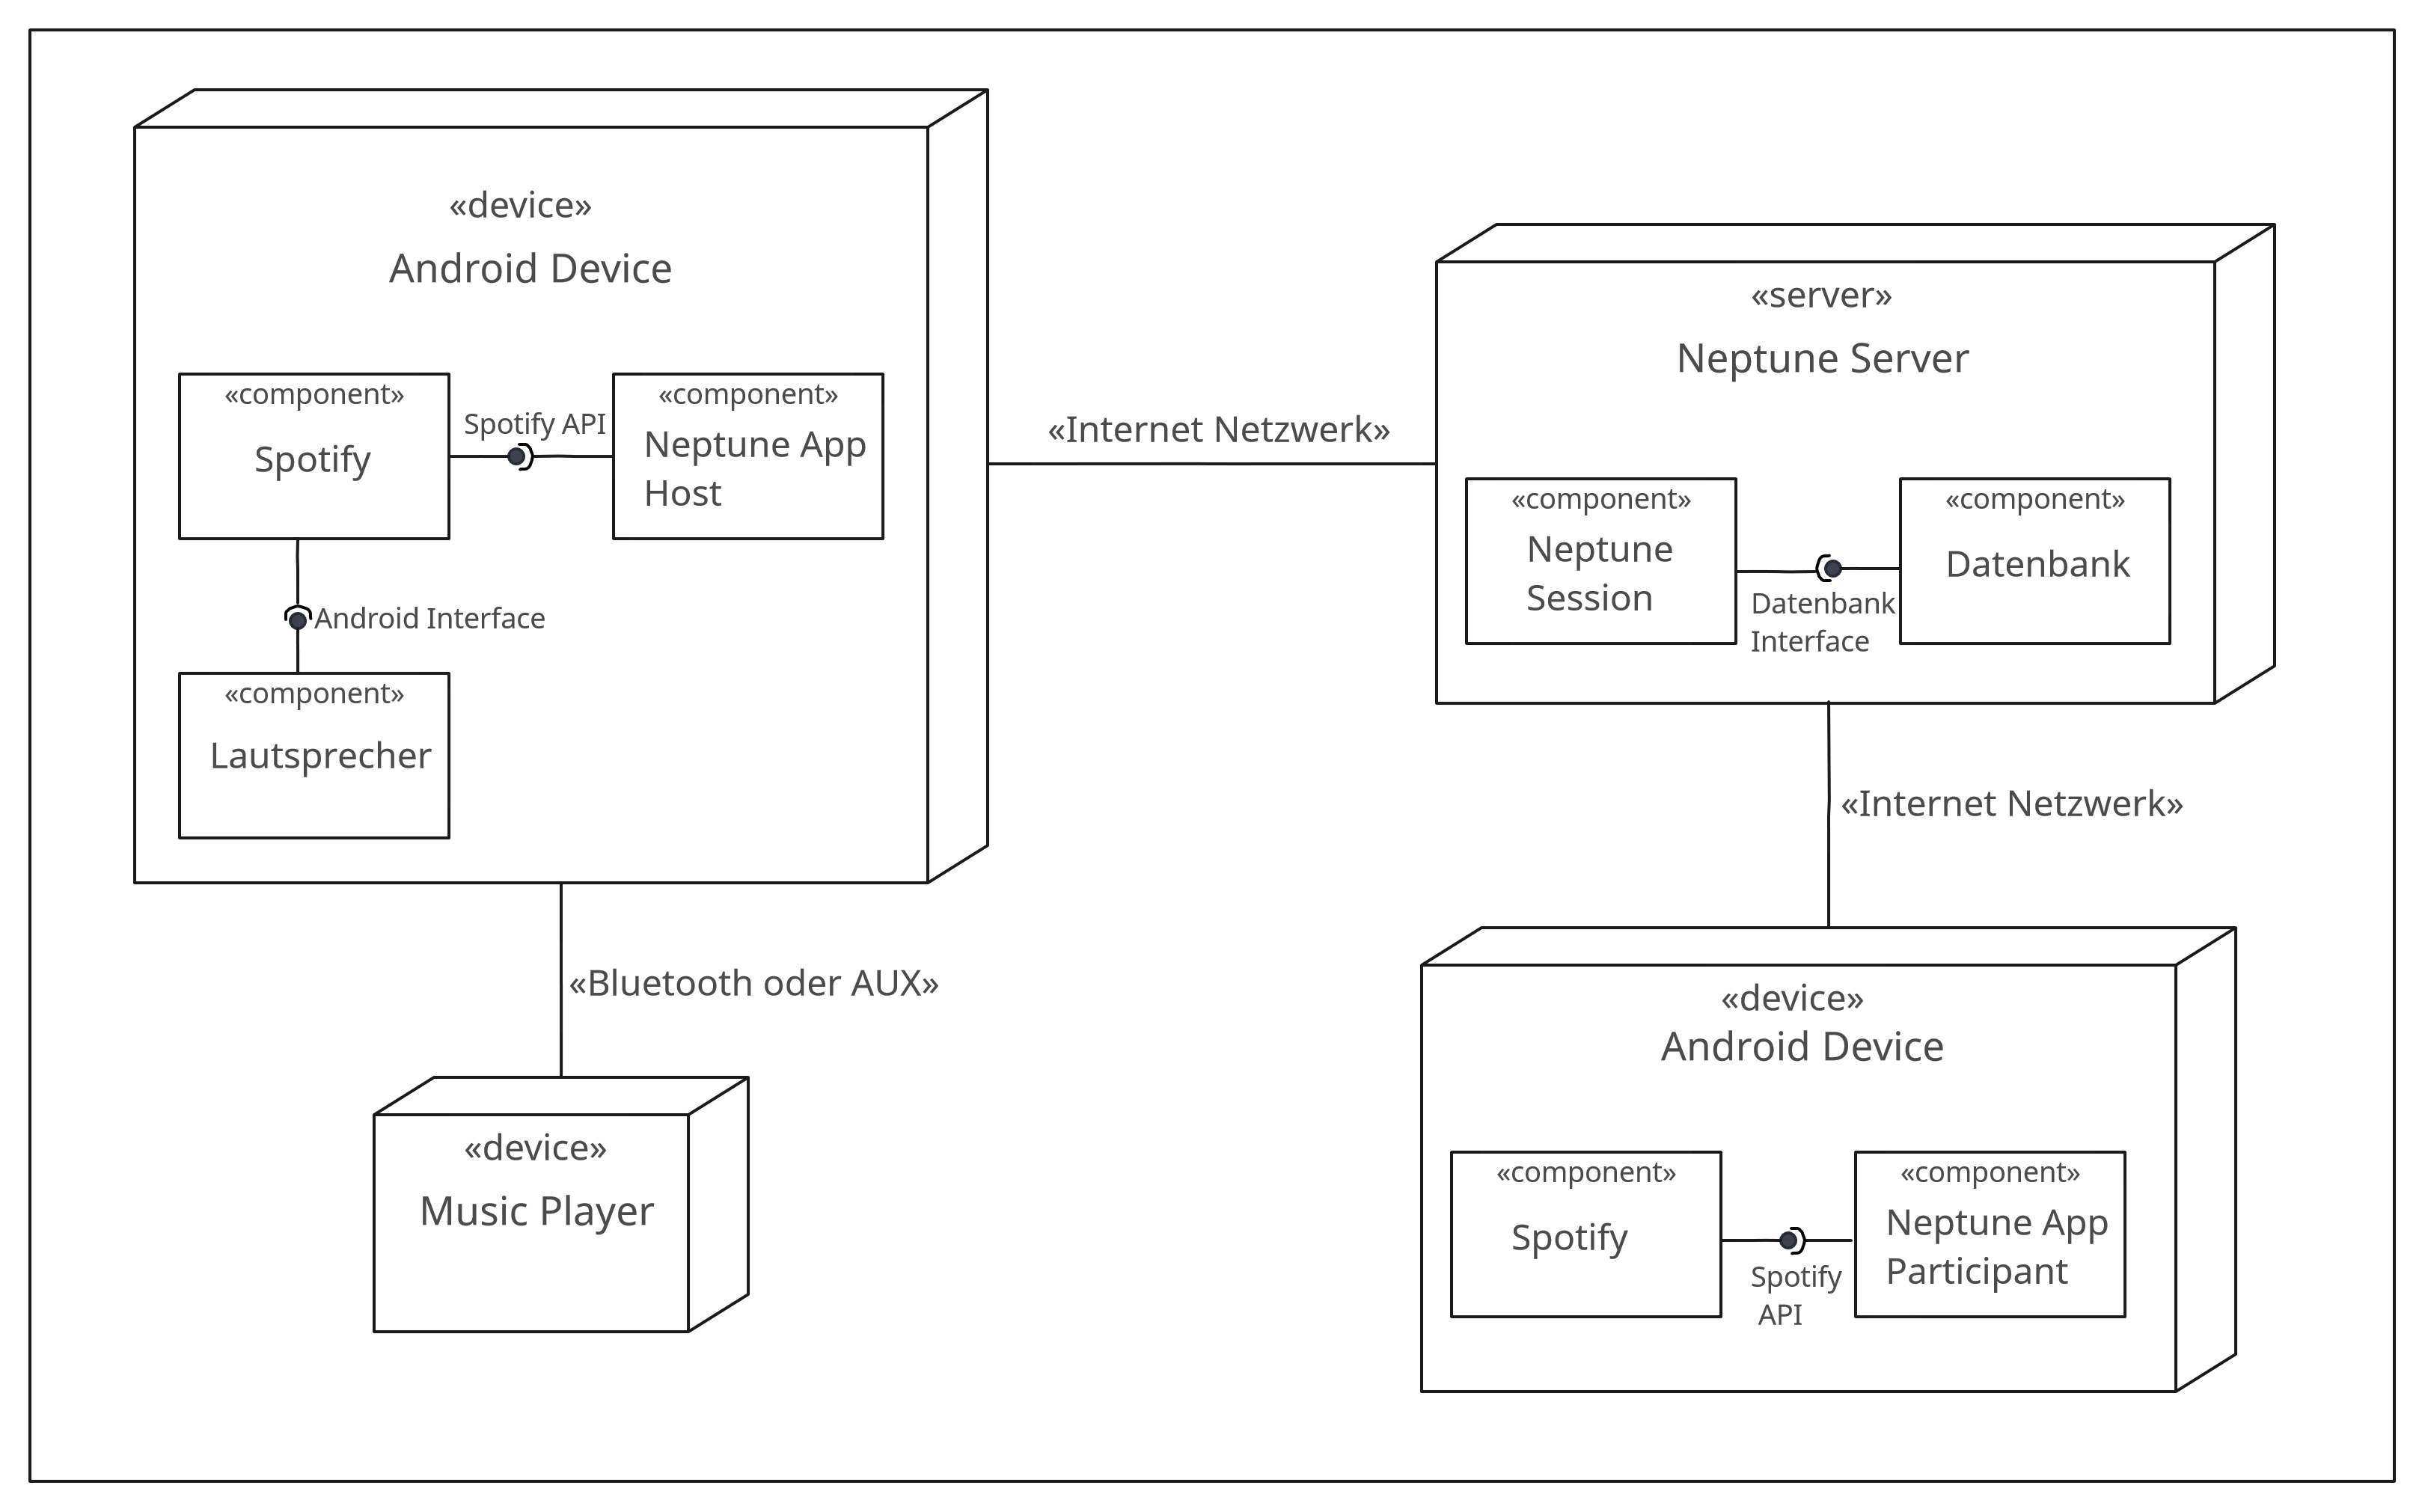
\includegraphics[width = 16cm]{LATEX/Pflichtenheft/GraphicDesigns/Verteilungsdiagramm.png}
    \caption{Verteilungsdiagramm}
    \label{fig:Verteilungsdiagramm}
\end{figure}



\chapter{Produktdaten}
\label{chap:Produktdaten}

\section{Systemdaten}
\label{sec:Produktdaten:Systemdaten}

Als Systemdaten werden sämtliche Daten zur Generierung der Benutzeroberfläche gespeichert, sowie die eindeutige Identifikation der App und Daten zum Auffinden des Servers. Zustandsdaten der App werden je nach Entwurfsentscheidung abgespeichert, um die App auch nach dem Schließen im selben Zustand erneut laden zu können. Es werden keinerlei Benutzereinstellungen oder Historiendaten gespeichert (SICHER ???). Auf dem Server werden Daten zum Zustand von Sessions gespeichert. Diese Session-Daten oder Teile von ihnen können auch kurzfristig lokal in der App der User gespeichert werden.

\section{Nutzerdaten}
\label{sec:Produktdaten:Nutzerdaten}

Es werden keinerlei sensiblen Nutzerdaten gespeichert. Im Fall des Musikdienstes Spotify müssen zur Verwendung der API keine Nutzerdaten gespeichert werden. Nur der generierte Nutzungstoken der API wird lokal gespeichert. Außerdem wird nach der Installation eine eindeutige Identifikation der App generiert, um User voneinander zu unterscheiden. Diese Identifikation wird lokal gespeichert und bei der Kommunikation von App und Server verwendet.



\chapter{Anforderungen an die App-Umgebung}
\label{chap:Appumgebung}

Wir stellen folgen Software und Hardware-Anforderungen an die App-Umgebung:

\begin{itemize}
    \item Als Gerät wird ein Smartphone oder gleichwertiges Gerät mit mindestens Android 7.0 benötigt.
    \item Eine jederzeit aktive Internetverbindung wird zur Nutzung der App-Funktionalität benötigt.
    \item Ein verknüpfter Spotify-Account wird benötigt, um als Full Participant an einer Session teilzunehmen.
    \item Ein verknüpfter Spotify-Premium-Account wird benötigt, um als Host eine Session zu erstellen und an ihr teilzunehmen.
\end{itemize}




\chapter{Tools und Ressourcen zur Entwicklung}
\label{chap:Entwicklungsumgebung}

\section{Software}
\label{sec:Entwicklungsumgebung:Software}

\begin{itemize}
    \item Entwicklung
    \begin{itemize}
        \item Android Studio Giraffe (2022.3.1)
    \end{itemize}
    
    \item Versionsverwaltung
    \begin{itemize}
        \item Git
        \item GitHub (zur Kommunikation)
    \end{itemize}

    \item UML Modellierung (KOMMT SO EIN ZEUG DA JETZT REIN ???)
    \begin{itemize}
        \item Creately
    \end{itemize}

    \item Grafikentwürfe
    \begin{itemize}
        \item PHPStorm
        \item GIMP
    \end{itemize}

    \item Sonstige Software
    \begin{itemize}
        \item Overleaf (für LATEX Dokumentation)
    \end{itemize}
    
\end{itemize}

\section{Hardware}
\label{sec:Entwicklungsumgebung:Hardware}

\begin{itemize}
    \item Diverse handelsübliche PCs und Laptops
    \item Diverse Android Smartphones mit mindestens Android 7.0
    \item Linux Rootserver
\end{itemize}



\chapter{Begriffserklärungen}
\label{chap:Begriffserklärungen}

\textbf{App}
 - Der Teil des Softwaresystems, der auf dem Android-Gerät des Nutzers läuft.

 \textbf{Full Participant}
 - Mit dem Musikdienst verknüpfter Participant, der Tracks im gesamten Katalog des Musikdienstes suchen kann.

\textbf{Host}
 - Ersteller einer Session, der (vorgeschlagene) Musik abspielt (kein Participant). Der Host benötigt ein Premium Abonnenment des Musikdienstes Spotify.

 \textbf{Musikdienst}
 - Der Musik-Streaminganbieter, über den die App Musik abspielt. Bei dieser App ist das Spotify.

 \textbf{Participant}
 - Teilnehmer einer Session (nicht der Host). Überbegriff für Full Participant und Restricted Participant.

 \textbf{Produkt}
 - Der Zustand, in dem das System nach Fertigstellung sein wird.

 \textbf{Queue}
 - Liste von Liedern, welche als nächstes durch den Musikdienst abgespielt werden.

 \textbf{Restricted Participant}
 - Nicht mit dem Musikdienst verknüpfter Participant, der nur Tracks von den bisher upgevoteten suchen kann.

 \textbf{Server}
 - Der Teil des Softwaresystems, der nicht auf dem Android-Gerät des Nutzers, sondern auf einem zentralen und externen Server läuft.

 \textbf{Session}
 - Eine Gruppe aus Participants und einem Host. In ihr können Tracks upgevotet und vom Host abgespielt werden.

\textbf{System}
 - Das gesamte zu entwickelnde Softwaresystem, Überbegriff von App und Server.

 \textbf{Track}
 - Lied bzw. Musikstück.

 \textbf{Upvote}
 - Bewertung auf einen Track. Je mehr Upvotes ein Track hat, desto beliebter ist er.

 \textbf{User}
 - Jeder Benutzer der App, Participant und Host sind User.

 \textbf{Vorschlagsliste}
 - Liste von Tracks einer Session, die mindestens ein Upvote haben. Ausgenommen ist der Playlist-Modus: In diesem ist die Vorschlagsliste gleichbedeutend mit der eingestellten Playlist.
 

\end{document}
